%!TEX TS-program = xelatex
%!TEX encoding = UTF-8 Unicode

%!TEX TS-program = xelatex
%!TEX encoding = UTF-8 Unicode

% Author: Romain "Artefact2" Dal Maso <artefact2@gmail.com>
%
% This program is free software. It comes without any warranty, to the
% extent permitted by applicable law. You can redistribute it and/or
% modify it under the terms of the Do What The Fuck You Want To Public
% License, Version 2, as published by Sam Hocevar. See
% http://sam.zoy.org/wtfpl/COPYING for more details.

\ifdefined\isdraft
\documentclass[10pt,a4paper,draft,showtrims,openany]{memoir}
\else
\documentclass[10pt,a4paper,openany]{memoir}
\fi
\usepackage{xltxtra}
\usepackage{fontspec}
\usepackage{xunicode}
\usepackage[table]{xcolor}
\usepackage{everypage}
\usepackage{calc}
\usepackage[absolute]{textpos}
\usepackage{lettrine}
\usepackage[hidelinks,xetex]{hyperref}
\usepackage{lipsum}
\usepackage{environ}
\usepackage[nomessages]{fp}
\usepackage{multirow,makecell}
\usepackage{dblfloatfix}
\usepackage{multicol}

\definecolor{chapter}{RGB}{88, 23, 13}
\definecolor{subsecrule}{RGB}{211, 169, 98}
\definecolor{footer}{RGB}{128, 110, 76}
\definecolor{note}{RGB}{224, 229, 193}

%!TEX TS-program = xelatex
%!TEX encoding = UTF-8 Unicode

% Author: Romain "Artefact2" Dal Maso <artefact2@gmail.com>
% 
% This program is free software. It comes without any warranty, to the
% extent permitted by applicable law. You can redistribute it and/or
% modify it under the terms of the Do What The Fuck You Want To Public
% License, Version 2, as published by Sam Hocevar. See
% http://sam.zoy.org/wtfpl/COPYING for more details.

\setmainfont[
  Path = ./assets/fonts/,
  Extension = .otf,
  UprightFont = *,
  BoldFont = * Bold,
  ItalicFont = * Italic,
  BoldItalicFont = * Bold Italic,
]{Bookinsanity}

\newfontface\mreaves[
  Path = ./assets/fonts/,
  Extension = .otf,
  UprightFont = *-Fixed,
  LetterSpace = -3,
]{Mr Eaves Small Caps}

\newfontface\solberaimitation[
  Path = ./assets/fonts/,
  Extension = .otf,
  UprightFont = *,
]{Solbera Imitation}

\newfontfamily\nodesto[
  Path = ./assets/fonts/,
  Extension = .otf,
  UprightFont = *,
  BoldFont = * Bold,
  ItalicFont = * Italic,
  BoldItalicFont = * Bold Italic,
]{Nodesto Caps Condensed}

\newfontfamily\scaly[
  Path = ./assets/fonts/,
  Extension = .otf,
  UprightFont = *,
  BoldFont = * Bold,
  ItalicFont = * Italic,
  BoldItalicFont = * Bold Italic,
  SmallCapsFont = * Caps,
  SmallCapsFeatures = {LetterSpace = 4},
  BoldFeatures = {SmallCapsFont = * Caps Bold},
  ItalicFeatures = {SmallCapsFont = * Caps Italic},
  BoldItalicFeatures = {SmallCapsFont = * Caps Bold Italic},
]{Scaly Sans}

% The main font doesn't have whatever itemize uses by default.
% How many levels are there?
\renewcommand*{\labelitemi}{$—$}
\renewcommand*{\labelitemii}{\labelitemi}
\renewcommand*{\labelitemiii}{\labelitemi}
\renewcommand*{\labelitemiv}{\labelitemi}

%!TEX TS-program = xelatex
%!TEX encoding = UTF-8 Unicode

% Author: Romain "Artefact2" Dal Maso <artefact2@gmail.com>
%
% This program is free software. It comes without any warranty, to the
% extent permitted by applicable law. You can redistribute it and/or
% modify it under the terms of the Do What The Fuck You Want To Public
% License, Version 2, as published by Sam Hocevar. See
% http://sam.zoy.org/wtfpl/COPYING for more details.

% Parts
\newcommand*{\hbPartCover}{assets/samples/part-cover}
\newcommand*{\hbPartSubcover}{assets/samples/part-cover2}

\renewcommand*{\thepart}{\arabic{part}}
\renewcommand*{\beforepartskip}{\null\vspace*{-55pt}\hspace*{-10pt}}
%\renewcommand*{\afterpartskip}{\clearpage\hbFullPageArtHook{\hbPartSubcover}}
\renewcommand*{\printpartname}{\AddThispageHook{%
    \thispagestyle{part}%
    \begin{tb*}{\paperwidth}{0pt}{0pt}%
      \includegraphics[width=\paperwidth,height=\paperheight]{\hbPartCover}
    \end{tb*}%
    \begin{tb*}{\paperwidth}{0pt}{0pt}%
      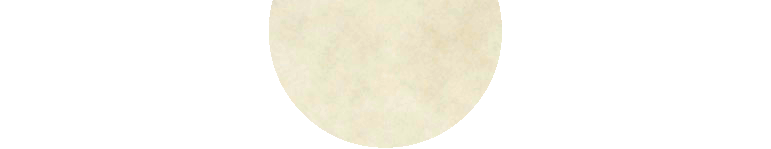
\includegraphics[width=\paperwidth]{assets/header-part-circ}
    \end{tb*}%
    \begin{tb*}{.5\paperwidth}{0pt}{0pt}%
      
\includegraphics[width=.5\paperwidth]{assets/header-part}
    \end{tb*}%
    \begin{tb*}{.5\paperwidth}{.5\paperwidth}{0pt}
      \reflectbox{
\includegraphics[width=.5\paperwidth]{assets/header-part}}
    \end{tb*}%
  }%
  \hspace*{-8pt}\nodesto\fontsize{64pt}{64pt}\selectfont\color{chapter}PART%
}
\renewcommand*{\printpartnum}{\nodesto\fontsize{64pt}{64pt}\selectfont\color{chapter}\!\thepart}
\renewcommand*{\parttitlefont}{\color{chapter}\Large\scaly\bfseries\vspace*{-18pt}\hspace*{-8pt}}

% Chapters
\newcommand*{\hbChapterHeader}{\AddThispageHook{%
    \begin{tb*}{.5\paperwidth}{0pt}{0pt}%
      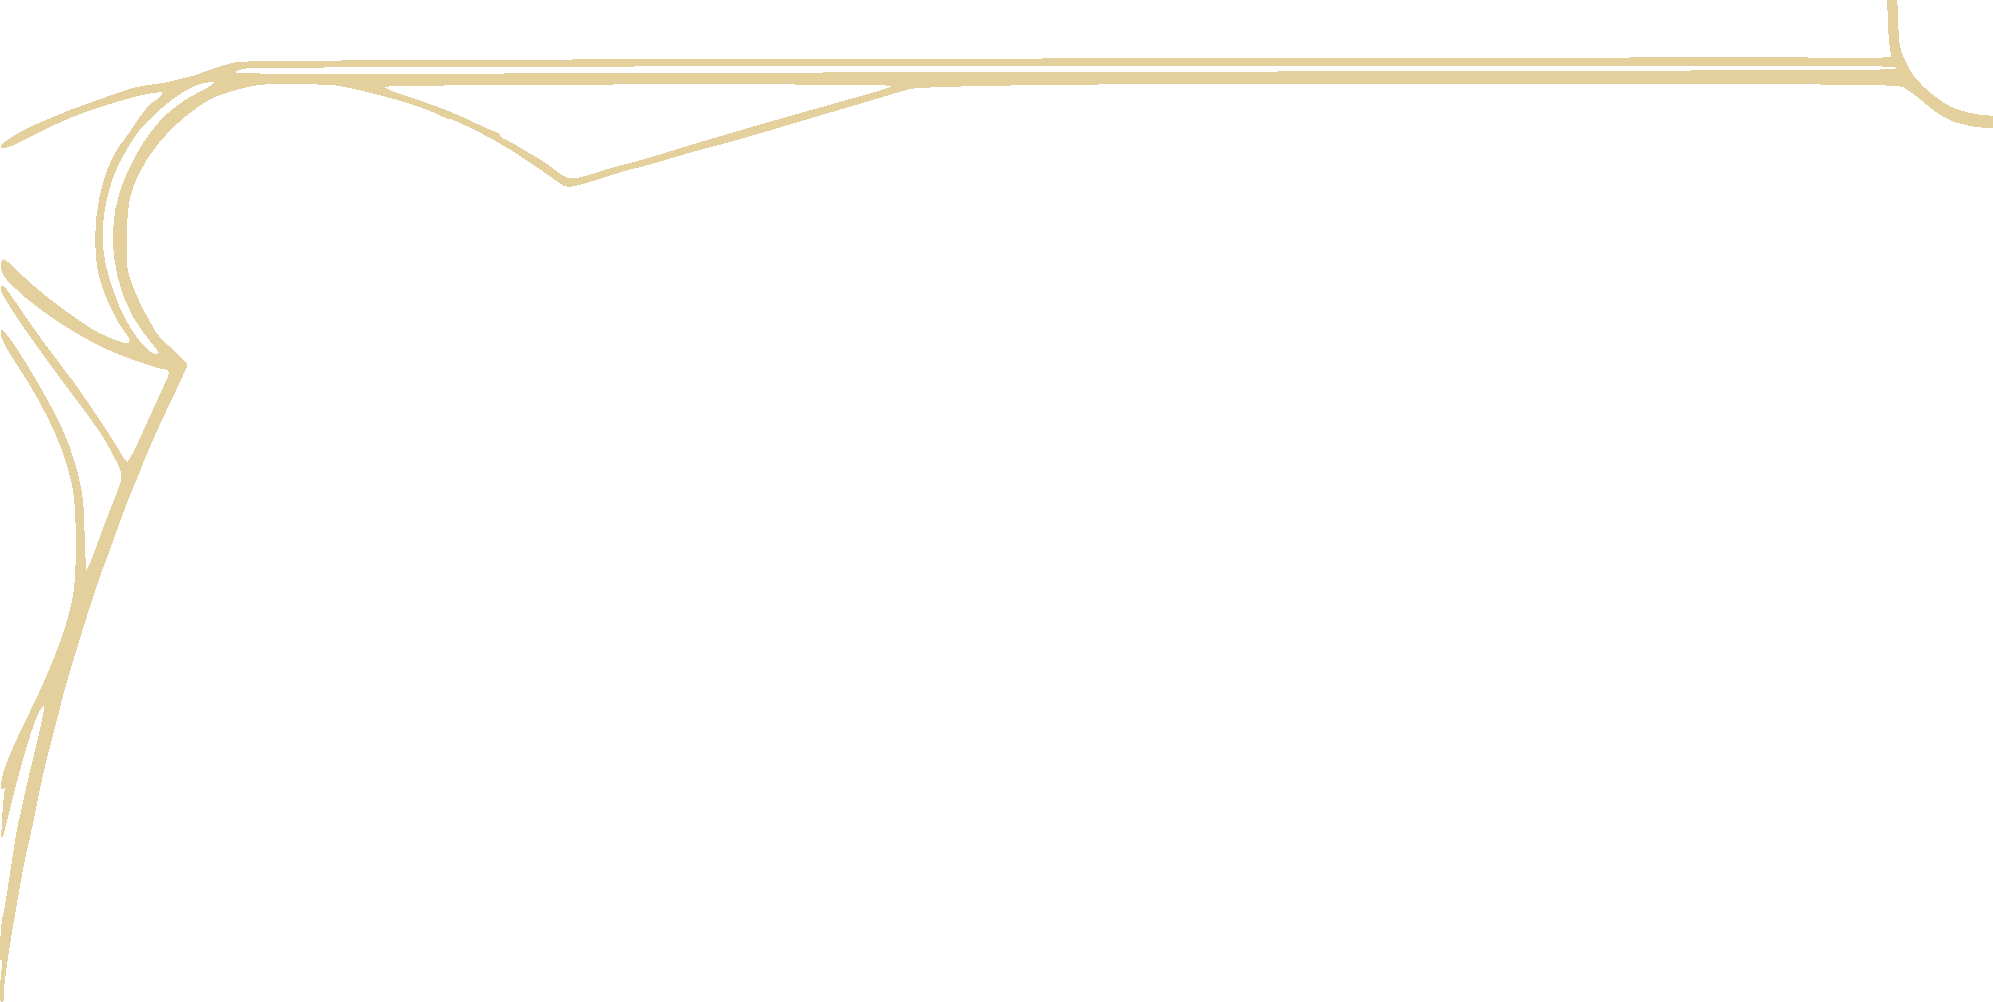
\includegraphics[width=.5\paperwidth]{assets/header-chapter}
    \end{tb*}%
    \begin{tb*}{.5\paperwidth}{.5\paperwidth}{0pt}%
      \reflectbox{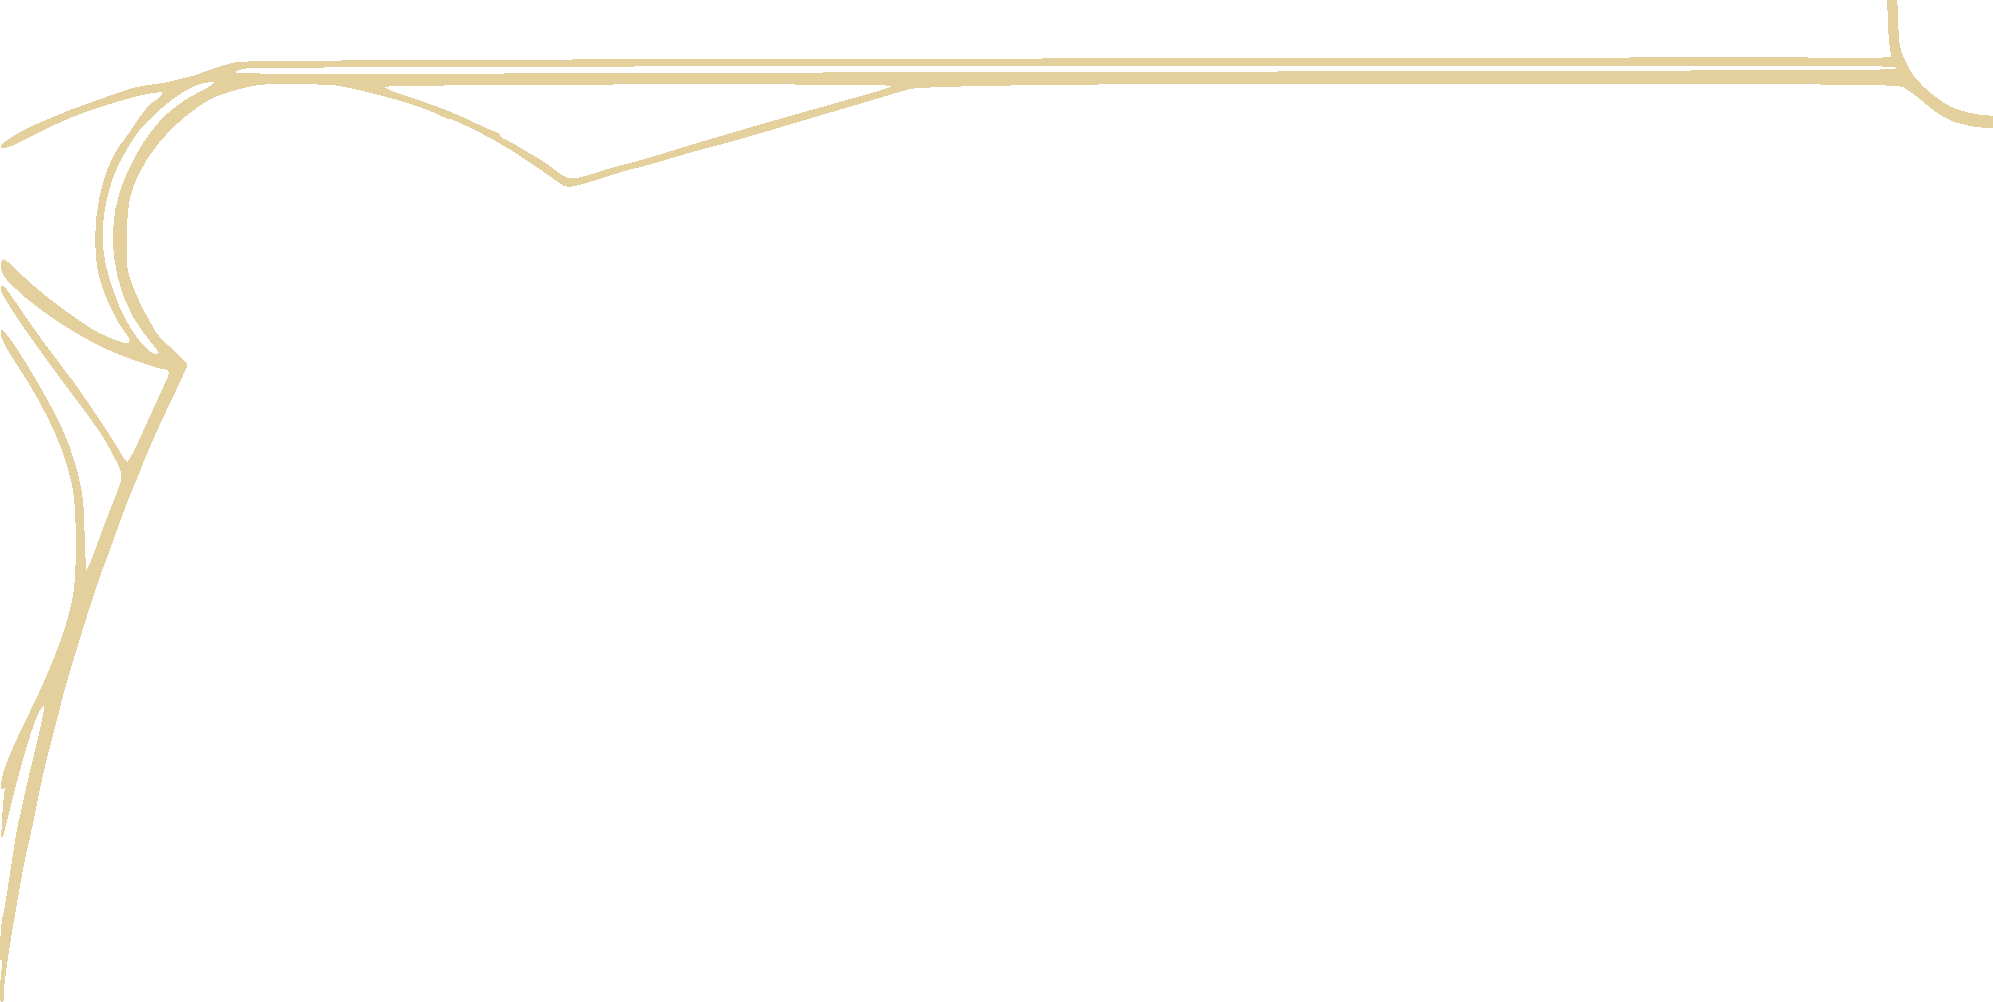
\includegraphics[width=.5\paperwidth]{assets/header-chapter}}
    \end{tb*}%
  }%
}
\renewcommand*{\chaptitlefont}{\color{chapter}\HUGE\mreaves\raggedright}
\renewcommand*{\printchaptername}{}
\renewcommand*{\chapternamenum}{}
\renewcommand*{\chapnumfont}{\chaptitlefont}
\makeatletter
\renewcommand*{\printchapternum}{\hbChapterHeader\chapnumfont \@chapapp\space\thechapter:\space}
\makeatother
\renewcommand*{\afterchapternum}{}
\renewcommand*{\printchapternonum}{\hbChapterHeader}
\renewcommand*{\beforechapskip}{0pt}
\renewcommand*{\afterchapskip}{\aftersecskip}

\newcommand*{\hbRootChapter}[1]{%
  \chapter*{#1}
  \addcontentsline{toc}{part}{#1}
  \markboth{#1}{#1}
}

\newcommand*{\hbAppendix}{%
  \appendix%
  \makepsmarks{hbRegular}{%
    \renewcommand*{\chaptermark}[1]{\markboth{appendix \alph{chapter}\space\rule{1pt}{.4\baselineskip}\space\MakeLowercase{####1}}{appendix \alph{chapter}\space\rule{1pt}{.4\baselineskip}\space\MakeLowercase{####1}}}%
    \renewcommand*{\sectionmark}[1]{}%
  }%
  \addcontentsline{toc}{part}{Appendix}%
  \pagestyle{hbRegular}%
}

\newcommand*{\hbFakeToc}[3]{}
%\newcommand*{\hbRootAppendix}[1]{%
%  \let\hbRealToc=\addcontentsline%
%  \let\addcontentsline=\hbFakeToc%
%  \chapter{#1}
%  \let\addcontentsline=\hbRealToc%
%  \addcontentsline{toc}{part}{Appendix\space\thechapter:\space#1}
%  \markboth{#1}{#1}
%}
\newcommand*{\hbRootAppendix}[1]{%
  \chapter{#1}
  \markboth{#1}{#1}
}

% Sections
\setsecnumformat{}
\setsecheadstyle{\color{chapter}\Huge\mreaves\raggedright}

% Subsections
\newcommand{\ruledsubsec}[1]{%
  \noindent\begin{minipage}{\linewidth}%
    \color{chapter}\huge\mreaves\raggedright #1%
    \par\vspace{-\prevdepth}\vspace{1pt}\color{subsecrule}\rule[\baselineskip]{\linewidth}{1pt}\vspace{-\baselineskip}\vspace{2pt}%
  \end{minipage}%
}
\setsubsecheadstyle{\ruledsubsec}
\renewcommand*{\aftersubsecskip}{.1\baselineskip}

% Subsubsections
\setsubsubsecheadstyle{\color{chapter}\LARGE\mreaves}
\renewcommand*{\aftersubsubsecskip}{\aftersubsecskip}

% Paragraphs and subparagraphs
\setafterparaskip{-3pt}
\setaftersubparaskip{-3pt}

% Table of Contents
\twocoltocetc
\renewcommand*{\cftsectiondotsep}{0.5}

\renewcommand*{\cftpartfont}{\color{chapter}\LARGE\mreaves}

\newsavebox{\hbPartname}
\newlength{\hbPartnamew}
\sbox{\hbPartname}{\cftpartfont Part\space}
\settowidth{\hbPartnamew}{\usebox{\hbPartname}}
\renewcommand*{\cftpartname}{\usebox{\hbPartname}}

\renewcommand*{\cftpartaftersnum}{:\space}
\renewcommand*{\cftpartafterpnum}{\par\vspace{-\prevdepth}\vspace{1pt}\color{subsecrule}\hspace{-\cftpartnumwidth}\hspace{-\hbPartnamew}\hspace{-\cftpartindent}\rule[\baselineskip]{\linewidth}{1pt}\vspace*{-\baselineskip}\vspace{2pt}}
\renewcommand*{\cftbeforepartskip}{10pt}
\renewcommand*{\cftpartnumwidth}{15pt}

\renewcommand*{\cftchapterfont}{\color{chapter}\Large\mreaves}
\renewcommand*{\cftchaptername}{Chapter\space}
\renewcommand*{\cftappendixname}{Appendix\space}
\renewcommand*{\cftchapteraftersnum}{:\space}
\renewcommand*{\cftchapterindent}{10pt}
\renewcommand*{\cftbeforechapterskip}{5pt}

\renewcommand*{\cftsectionnumwidth}{0pt}
\renewcommand*{\cftsectionpresnum}{\fontsize{1sp}{0}\selectfont} % XXX
\renewcommand*{\cftsectionindent}{20pt}

\renewcommand*{\cfttabledotsep}{0.5}
\renewcommand*{\cfttablenumwidth}{0pt}
\renewcommand*{\cfttablepresnum}{\fontsize{1sp}{0}\selectfont} % XXX
\renewcommand*{\cfttableindent}{0pt}

% Cover page
\newcommand*{\hbCover}{assets/cover}
\newcommand*{\hbSubcover}{assets/cover2}
\newcommand{\hbTitle}{Title. Renew me!}
\newcommand{\hbSubtitle}{Subtitle. Renew me!}

\newcommand{\hbMakecover}{
  \onecolumn%
  \thispagestyle{empty}%
  \AddThispageHook{%
    \begin{tb*}{\paperwidth}{0pt}{0pt}%
      \includegraphics[width=\paperwidth,height=\paperheight]{\hbCover}
    \end{tb*}%
  }%
  \begin{center}%
    \vspace*{-15mm}
\includegraphics[width=3cm]{assets/dnd-logo-initials}\\*\vspace*{15mm}%
    \nodesto%
    \fontsize{48pt}{48pt}\selectfont%
    \fillstroke{[1]}{[0]}{1.5}{\MakeUppercase\hbTitle}\\*%
    \normalfont\normalsize
\includegraphics[width=.5\paperwidth]{assets/separator}%
    \LARGE\vfill%
    % XXX: font doesn't look right
    \fillstroke{[1]}{[0]}{.5}{\textbf{\hbSubtitle}}%
  \end{center}%
  \clearpage%
  \twocolumn%
}

\newcommand{\hbMakesubcover}{%
  \onecolumn%
  \thispagestyle{empty}%
  \AddThispageHook{
    \begin{tb*}{\paperwidth}{0pt}{0pt}%
      \includegraphics[width=\paperwidth,height=\paperheight]{\hbSubcover}
    \end{tb*}%
  }%
  \begin{center}%
    \nodesto%
    \fontsize{48pt}{48pt}\selectfont%
    \MakeUppercase\hbTitle\\*%
    \normalfont\normalsize
\includegraphics[width=.5\paperwidth]{assets/separator}%
    \LARGE\vfill%
    
\includegraphics[width=1.5cm]{assets/dnd-logo-amp}%
  \end{center}%
  \clearpage%
  \twocolumn%
}

%!TEX TS-program = xelatex
%!TEX encoding = UTF-8 Unicode

% Author: Romain "Artefact2" Dal Maso <artefact2@gmail.com>
%
% This program is free software. It comes without any warranty, to the
% extent permitted by applicable law. You can redistribute it and/or
% modify it under the terms of the Do What The Fuck You Want To Public
% License, Version 2, as published by Sam Hocevar. See
% http://sam.zoy.org/wtfpl/COPYING for more details.

\NewEnviron{tb*}[3]{%
\begin{textblock*}{#1}(\ox+#2,\oy+#3)\BODY\end{textblock*}%
}

\NewEnviron{rtb*}[3]{%
\TPoptions{absolute=false}%
\begin{textblock*}{#1}(#2,#3)\BODY\end{textblock*}%
\TPoptions{absolute=true}%
}

\newcommand*{\fakeminipage}[1]{%
\begin{minipage}[b]{0pt}%
\setlength{\vfuzz}{\stockwidth}%
\setlength{\hfuzz}{\stockheight}%
#1\end{minipage}%
\setlength{\vfuzz}{0pt}%
\setlength{\hfuzz}{0pt}%
}

\newlength{\ox}
\newlength{\oy}

\ifdefined\isdraft
\stockaiii
\pageaiv
\setlength{\ox}{.5\stockwidth-.5\paperwidth}
\setlength{\oy}{.5\stockheight-.5\paperheight}
\settrims{\oy}{\ox}
\else
\pageaiv
\setlength{\ox}{0pt}
\setlength{\oy}{0pt}
\fi

\setulmarginsandblock{16mm}{20mm}{1}
\setlrmarginsandblock{20mm}{16mm}{1}
\setcolsepandrule{8mm}{0mm}
\setheadfoot{10mm}{\paperheight-\uppermargin-\textheight-6mm}
\setheaderspaces{*}{0mm}{*}
\settypeoutlayoutunit{mm}
\checkandfixthelayout

\setlength{\multicolsep}{0pt} % XXX may have bad side effects?
\frenchspacing

% XXX why is this breaking \twocolumn (will reset to one after a part) ?
\newcommand*{\hbBackground}{assets/background}
\AddEverypageHook{\begin{tb*}{\paperwidth}{0pt}{0pt}%
    \includegraphics[width=\paperwidth,height=\paperheight]{\hbBackground}%
\end{tb*}\twocolumn}

\makepagestyle{hbRegular}
\aliaspagestyle{chapter}{hbRegular}
\aliaspagestyle{part}{hbRegular}

\makeoddfoot{hbRegular}{%
  \raisebox{-9mm}{\fakeminipage{\hspace*{-\spinemargin}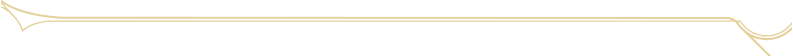
\includegraphics[width=\paperwidth]{assets/footer}}}%
}{}{%
  \color{footer}\mreaves \rightmark \hspace*{20mm}\hspace*{-\foremargin} \\[-2mm]
  \begin{minipage}{1cm}\centering\Large\thepage\end{minipage}\hspace*{2pt}\hspace*{-\foremargin}
}
\makeevenfoot{hbRegular}{%
  \color{footer}\mreaves \hspace*{20mm}\hspace*{-\foremargin} \leftmark \\[-2mm]
  \hspace*{-\foremargin}\hspace*{5pt}\begin{minipage}{1cm}\centering\Large\thepage\end{minipage}
}{}{%
  \raisebox{-9mm}{\fakeminipage{%
    \hspace*{-\paperwidth}\hspace*{\spinemargin}%
    \reflectbox{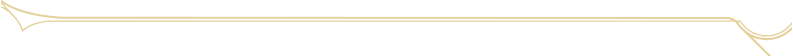
\includegraphics[width=\paperwidth]{assets/footer}}%
  }}%
}

\makepsmarks{hbRegular}{
\renewcommand*{\partmark}[1]{\markboth{part \thepart\space\rule{1pt}{.4\baselineskip}\space\MakeLowercase{##1}}{part \thepart\space\rule{1pt}{.4\baselineskip}\space\MakeLowercase{##1}}}
\renewcommand*{\chaptermark}[1]{\partmark{##1}}
\renewcommand*{\sectionmark}[1]{}
}

\pagestyle{hbRegular}

%!TEX TS-program = xelatex
%!TEX encoding = UTF-8 Unicode

% Author: Romain "Artefact2" Dal Maso <artefact2@gmail.com>
% 
% This program is free software. It comes without any warranty, to the
% extent permitted by applicable law. You can redistribute it and/or
% modify it under the terms of the Do What The Fuck You Want To Public
% License, Version 2, as published by Sam Hocevar. See
% http://sam.zoy.org/wtfpl/COPYING for more details.

\newlength{\hbNoteCurparskip}
\newlength{\hbNoteCurparindent}
\newlength{\hbNotePrevSubsubsectionSkip}
\newlength{\hbNotePrevParagraphSkip}
\newlength{\hbNoteBW}
\newlength{\hbNoteBH}
\newlength{\hbNoteRW}
\newlength{\hbNotePS}
\newlength{\hbNotePadding}
\newlength{\hbNoteBoxWidth}
\newlength{\hbNoteBoxHeight}
\newlength{\hbNoteBoxDepth}
\newsavebox{\hbNoteBox}

\setlength{\hbNoteBW}{1pt} % Border width for note
\setlength{\hbNoteBH}{6pt} % Border height for note
\setlength{\hbNoteRW}{1pt} % Rule width for note2
\setlength{\hbNotePS}{3pt} % Point corner for note2
\setlength{\hbNotePadding}{2pt} % Horizontal padding inside notes

\newcommand*{\hbNotePrevSubsubsectionStyle}{}
\newcommand*{\hbNotePrevParagraphStyle}{}

\newcommand*{\hbNoteBefore}{%
  \setlength{\hbNoteCurparskip}{\parskip}%
  \setlength{\hbNoteCurparindent}{\parindent}%
  \renewcommand*{\hbNotePrevSubsubsectionStyle}{\subsubsecheadstyle}%
  \renewcommand*{\hbNotePrevParagraphStyle}{\paraheadstyle}%
  \setlength{\hbNotePrevSubsubsectionSkip}{\beforesubsubsecskip}%
  \setlength{\hbNotePrevParagraphSkip}{\beforeparaskip}%
  \setsubsubsecheadstyle{\scaly\large\bfseries\scshape}%
  \setparaheadstyle{\scaly\bfseries}%
  \setbeforesubsubsecskip{0pt}%
  \setbeforeparaskip{0pt}%
}

\newcommand*{\hbNoteAfter}{%
  \setsubsubsecheadstyle{\hbNotePrevSubsubsectionStyle}%
  \setparaheadstyle{\hbNotePrevParagraphStyle}%
  \setbeforesubsubsecskip{\hbNotePrevSubsubsectionSkip}%
  \setbeforeparaskip{\hbNotePrevParagraphSkip}%
}

% XXX where is that 1pt vertical offset FROM?!
\newcommand*{\hbNoteDraw}{%
  \settowidth{\hbNoteBoxWidth}{\usebox{\hbNoteBox}}%
  \settoheight{\hbNoteBoxHeight}{\usebox{\hbNoteBox}}%
  \settodepth{\hbNoteBoxDepth}{\usebox{\hbNoteBox}}%
  \TPoptions{absolute=false}%
  \noindent\vspace*{\hbNoteBH}\hspace*{\hbNoteBW}%
  \begin{textblock*}{\linewidth}(0pt,-\hbNoteBH+1pt)
    \scalebox{1}[-1]{
\includegraphics[width=1.307\hbNoteBH,height=\hbNoteBH]{assets/note-corner}}
  \end{textblock*}%
  \begin{textblock*}{\linewidth}(\hbNoteBoxWidth-1.307\hbNoteBH,-\hbNoteBH+1pt)
    \scalebox{-1}[-1]{
\includegraphics[width=1.307\hbNoteBH,height=\hbNoteBH]{assets/note-corner}}
  \end{textblock*}%
  \begin{textblock*}{\linewidth}(0pt,\hbNoteBoxHeight+\hbNoteBoxDepth+1pt)
    \scalebox{1}[1]{
\includegraphics[width=1.307\hbNoteBH,height=\hbNoteBH]{assets/note-corner}}
  \end{textblock*}%
  \begin{textblock*}{\linewidth}(\hbNoteBoxWidth-1.307\hbNoteBH,\hbNoteBoxHeight+\hbNoteBoxDepth+1pt)
    \scalebox{-1}[1]{
\includegraphics[width=1.307\hbNoteBH,height=\hbNoteBH]{assets/note-corner}}
  \end{textblock*}%
  \begin{textblock*}{\linewidth}(1.306\hbNoteBH,-\hbNoteBH+1pt)
    \scalebox{1}[-1]{
\includegraphics[width=\hbNoteBoxWidth-2.612\hbNoteBH,height=\hbNoteBH]{assets/note-bottom}}
  \end{textblock*}%
  \begin{textblock*}{\linewidth}(1.306\hbNoteBH,\hbNoteBoxHeight+\hbNoteBoxDepth+1pt)
    
\includegraphics[width=\hbNoteBoxWidth-2.612\hbNoteBH,height=\hbNoteBH]{assets/note-bottom}
  \end{textblock*}%
  \begin{textblock*}{\linewidth}(-\hbNoteBW,1pt)
    
\includegraphics[width=\hbNoteBW,height=\hbNoteBoxHeight+\hbNoteBoxDepth]{assets/note-side}
  \end{textblock*}%
  \begin{textblock*}{\linewidth}(\hbNoteBoxWidth,1pt)
    \reflectbox{
\includegraphics[width=\hbNoteBW,height=\hbNoteBoxHeight+\hbNoteBoxDepth]{assets/note-side}}
  \end{textblock*}%
  \usebox{\hbNoteBox}\vspace*{\hbNoteBH}%
  \TPoptions{absolute=true}%
}

\NewEnviron{hbNote}[1][h]{%
\hbNoteBefore%
\begin{figure}[#1]%
  \sbox{\hbNoteBox}{%
    \colorbox{note}{%
      \hspace*{\hbNotePadding}\begin{minipage}[b]{\linewidth-2\hbNotePadding-2\hbNoteBW-2\fboxsep}%
        \setlength{\parskip}{\hbNoteCurparskip}%
        \setlength{\parindent}{\hbNoteCurparindent}%
        \noindent\scaly\small\BODY%
      \end{minipage}%
      \hspace*{\hbNotePadding}%
    }%
  }%
  \hbNoteDraw%
\end{figure}%
\hbNoteAfter%
}

\NewEnviron{hbNoteWide}[1][t]{%
\hbNoteBefore%
\begin{figure*}[#1]%
  \sbox{\hbNoteBox}{%
    \colorbox{note}{%
      \hspace*{\hbNotePadding}\begin{minipage}[b]{\linewidth-2\hbNotePadding-2\hbNoteBW-2\fboxsep}%
        \setlength{\parskip}{\hbNoteCurparskip}%
        \setlength{\parindent}{\hbNoteCurparindent}%
        \noindent\scaly\small\BODY%
      \end{minipage}%
      \hspace*{\hbNotePadding}%
    }%
  }%
  \hbNoteDraw%
\end{figure*}%
\hbNoteAfter%
}

% XXX same
\newcommand*{\hbNoteDrawVar}{%
  \settowidth{\hbNoteBoxWidth}{\usebox{\hbNoteBox}}%
  \settoheight{\hbNoteBoxHeight}{\usebox{\hbNoteBox}}%
  \settodepth{\hbNoteBoxDepth}{\usebox{\hbNoteBox}}%
  \TPoptions{absolute=false}%
  \noindent\hspace*{\hbNoteRW}%
  \begin{textblock*}{\linewidth}(-.5\hbNoteRW,1pt-\hbNotePS)
  
\includegraphics[width=\hbNoteBoxWidth+\hbNoteRW,height=\hbNotePS]{assets/note-var-top}
  \end{textblock*}%
  \begin{textblock*}{\linewidth}(-.5\hbNoteRW,1pt+\hbNoteBoxHeight+\hbNoteBoxDepth)
  \scalebox{1}[-1]{
\includegraphics[width=\hbNoteBoxWidth+\hbNoteRW,height=\hbNotePS]{assets/note-var-top}}
  \end{textblock*}%
  \begin{textblock*}{\hbNotePS}(-.5\hbNotePS-.5\hbNoteRW,1pt-\hbNotePS)
  
\includegraphics[width=\hbNotePS,height=\hbNotePS]{assets/note-var-corner}
  \end{textblock*}%
  \begin{textblock*}{\hbNotePS}(\hbNoteBoxWidth+.5\hbNoteRW-.5\hbNotePS,1pt-\hbNotePS)
  
\includegraphics[width=\hbNotePS,height=\hbNotePS]{assets/note-var-corner}
  \end{textblock*}%
  \begin{textblock*}{\hbNotePS}(-.5\hbNotePS-.5\hbNoteRW,1pt+\hbNoteBoxHeight+\hbNoteBoxDepth)
  
\includegraphics[width=\hbNotePS,height=\hbNotePS]{assets/note-var-corner}
  \end{textblock*}%
  \begin{textblock*}{\hbNotePS}(\hbNoteBoxWidth+.5\hbNoteRW-.5\hbNotePS,1pt+\hbNoteBoxHeight+\hbNoteBoxDepth)
  
\includegraphics[width=\hbNotePS,height=\hbNotePS]{assets/note-var-corner}
  \end{textblock*}%
  \begin{textblock*}{\hbNoteRW}(-\hbNoteRW,1pt-.5\hbNotePS)
  {\color{chapter}\rule{\hbNoteRW}{\hbNoteBoxHeight+\hbNoteBoxDepth+\hbNotePS}}
  \end{textblock*}%
  \begin{textblock*}{\hbNoteRW}(\hbNoteBoxWidth,1pt-.5\hbNotePS)
  {\color{chapter}\rule{\hbNoteRW}{\hbNoteBoxHeight+\hbNoteBoxDepth+\hbNotePS}}
  \end{textblock*}%
  \usebox{\hbNoteBox}\hspace*{\hbNoteRW}%
  \TPoptions{absolute=true}%
}

\NewEnviron{hbNote2}[1][h]{%
\hbNoteBefore%
\begin{figure}[#1]%
  \sbox{\hbNoteBox}{%
    \colorbox{white}{%
      \hspace*{\hbNotePadding}\begin{minipage}[b]{\linewidth-2\hbNotePadding-2\hbNoteRW-2\fboxsep}%
        \setlength{\parskip}{\hbNoteCurparskip}%
        \setlength{\parindent}{\hbNoteCurparindent}%
        \noindent\scaly\small\BODY%
      \end{minipage}%
      \hspace*{\hbNotePadding}%
    }%
  }%
  \hbNoteDrawVar%
\end{figure}%
\hbNoteAfter%
}

\NewEnviron{hbNoteWide2}[1][t]{%
\hbNoteBefore%
\begin{figure*}[#1]%
  \sbox{\hbNoteBox}{%
    \colorbox{white}{%
      \hspace*{\hbNotePadding}\begin{minipage}[b]{\linewidth-2\hbNotePadding-2\hbNoteRW-2\fboxsep}%
        \setlength{\parskip}{\hbNoteCurparskip}%
        \setlength{\parindent}{\hbNoteCurparindent}%
        \noindent\scaly\small\BODY%
      \end{minipage}%
      \hspace*{\hbNotePadding}%
    }%
  }%
  \hbNoteDrawVar%
\end{figure*}%
\hbNoteAfter%
}

%!TEX TS-program = xelatex
%!TEX encoding = UTF-8 Unicode

% Author: Romain "Artefact2" Dal Maso <artefact2@gmail.com>
%
% This program is free software. It comes without any warranty, to the
% extent permitted by applicable law. You can redistribute it and/or
% modify it under the terms of the Do What The Fuck You Want To Public
% License, Version 2, as published by Sam Hocevar. See
% http://sam.zoy.org/wtfpl/COPYING for more details.

\newcommand*{\hbSBPrevdesclabel}{}
\newcommand*{\hbSBPrevsubsecstyle}{}
\newcommand*{\hbSBPrevsubsubsecstyle}{}
\newcommand*{\hbSBPrevparastyle}{}

\newlength{\hbSBPrevparaskip}
\newlength{\hbSBPrevsubsubsecskip}
\newlength{\hbSBPrevparaindent}

\newcommand*{\hbSBType}[1]{\textit{#1}}
\newcommand*{\hbSBSep}{%
  \leavevmode\\*%
  \noindent
\includegraphics[height=5pt,width=\linewidth]{assets/stat-block-separator}\\*%
  \noindent%
}
\newcommand*{\hbModifier}[1]{\FPeval{\result}{round((2*trunc(#1/2,0)-10)/2,0)}\ifnum\result>-1 +\result\else\result\fi}
\newcommand*{\hbSBAttributes}[6]{%
  {\color{chapter}%
  \begin{tabularx}{\linewidth}{@{}*{6}{>{\centering\arraybackslash}X@{}}}
    \textbf{STR} & \textbf{DEX} & \textbf{CON} & \textbf{INT} & \textbf{WIS} & \textbf{CHA} \\
    #1 (\hbModifier{#1}) & #2 (\hbModifier{#2}) & #3 (\hbModifier{#3}) & #4 (\hbModifier{#4}) & #5 (\hbModifier{#5}) & #6 (\hbModifier{#6})
  \end{tabularx}}%
}
\newcommand*{\hbSBsubsec}[1]{\color{chapter}\Huge\mreaves#1\vspace*{-2pt}}
\newcommand*{\hbSBsubsubsec}[1]{\color{chapter}\Large\scaly\scshape #1\par\vspace{-\prevdepth}\vspace{1pt}\hspace{-\parindent}\rule[\baselineskip]{\linewidth}{1pt}\vspace*{-\baselineskip}\vspace{2pt}}

\NewEnviron{hbStatBlockDescription}{%
  \renewcommand*{\hbSBPrevdesclabel}{\descriptionlabel}%
  \renewcommand*{\descriptionlabel}{\color{chapter}\hspace\labelsep\scaly\bfseries}%
  \begin{description}\tightlist\setlength{\labelsep}{3pt}\color{chapter}%
    \vspace*{-\topsep}\BODY\vspace*{-\topsep}%
  \end{description}%
  \renewcommand*{\descriptionlabel}{\hbSBPrevdesclabel}%
}

\NewEnviron{hbStatBlock}{%
  \renewcommand*{\hbSBPrevparastyle}{\paraheadstyle}%
  \renewcommand*{\hbSBPrevsubsecstyle}{\subsecheadstyle}%
  \renewcommand*{\hbSBPrevsubsubsecstyle}{\subsubsecheadstyle}%
  \setparaheadstyle{\scaly\small\bfseries}%
  \setsubsecheadstyle{\hbSBsubsec}%
  \setsubsubsecheadstyle{\hbSBsubsubsec}%
  \setlength{\hbSBPrevparaskip}{\beforeparaskip}%
  \setlength{\hbSBPrevsubsubsecskip}{\beforesubsubsecskip}%
  \setlength{\hbSBPrevparaindent}{\paraindent}%
  \setbeforeparaskip{.5em}%
  \setbeforesubsubsecskip{.5em}%
  \setparaindent{0pt}%
  \medbreak{\scaly\small\BODY}\medbreak%
  \setparaheadstyle{\hbSBPrevparastyle}%
  \setsubsecheadstyle{\hbSBPrevsubsecstyle}%
  \setsubsubsecheadstyle{\hbSBPrevsubsubsecstyle}%
  \setbeforeparaskip{\hbSBPrevparaskip}%
  \setbeforesubsubsecskip{\hbSBPrevsubsubsecskip}%
  \setparaindent{\hbSBPrevparaindent}
}

%!TEX TS-program = xelatex
%!TEX encoding = UTF-8 Unicode

% Author: Romain "Artefact2" Dal Maso <artefact2@gmail.com>
% 
% This program is free software. It comes without any warranty, to the
% extent permitted by applicable law. You can redistribute it and/or
% modify it under the terms of the Do What The Fuck You Want To Public
% License, Version 2, as published by Sam Hocevar. See
% http://sam.zoy.org/wtfpl/COPYING for more details.

\newcolumntype{L}{>{\small\scaly}l}
\newcolumntype{C}{>{\small\scaly}c}
\newcolumntype{R}{>{\small\scaly}r}
\newcolumntype{Y}{>{\small\scaly}X}
\newcolumntype{Z}{>{\small\scaly\centering\arraybackslash}X}

\newlength{\hbTableBorderX}
\newlength{\hbTableBorderY}
\newlength{\hbTableBorderS}
\newlength{\hbTableBoxWidth}
\newlength{\hbTableBoxHeight}
\newlength{\hbTableBoxDepth}
\newsavebox{\hbTableBox}

\setlength{\hbTableBorderX}{10pt}
\setlength{\hbTableBorderY}{14pt}
\setlength{\hbTableBorderS}{5em}

\renewcommand*{\arraystretch}{1.1}

\captionstyle{\raggedright}
\captiondelim{}
\captionnamefont{\fontsize{1sp}{0pt}\selectfont} % XXX: hackish
\captiontitlefont{\scaly\scshape\bfseries\large}

\newcommand*{\hbTableBefore}{%
  \global\rownum=0%
  \rowcolors{1}{}{note}%
}

\newcommand*{\hbTableDrawFancy}{%
    \settowidth{\hbTableBoxWidth}{\usebox{\hbTableBox}}%
    \settoheight{\hbTableBoxHeight}{\usebox{\hbTableBox}}%
    \settodepth{\hbTableBoxDepth}{\usebox{\hbTableBox}}%
    \TPoptions{absolute=false}%
    \noindent\vspace*{\hbTableBorderY}%
    \begin{textblock*}{\linewidth}(-\hbTableBorderX,-\hbTableBorderY)%
    \scalebox{-1}[1]{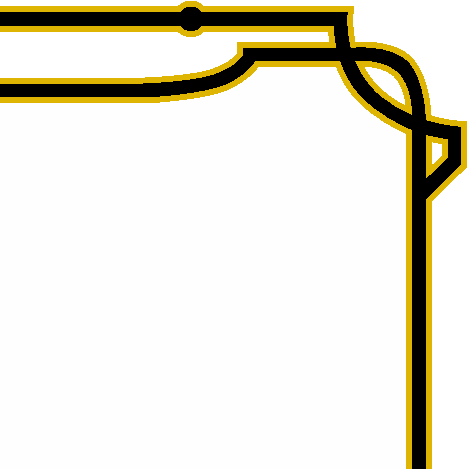
\includegraphics[width=\hbTableBorderS,height=\hbTableBorderS]{assets/fancy-table-corner}}
    \end{textblock*}%
    \begin{textblock*}{\linewidth}(\hbTableBoxWidth-\hbTableBorderS+\hbTableBorderX,-\hbTableBorderY)%
    \scalebox{1}[1]{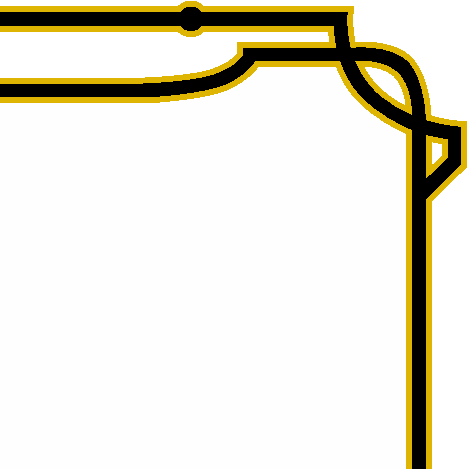
\includegraphics[width=\hbTableBorderS,height=\hbTableBorderS]{assets/fancy-table-corner}}
    \end{textblock*}%
    \begin{textblock*}{\linewidth}(-\hbTableBorderX,\hbTableBoxHeight+\hbTableBoxDepth-\hbTableBorderS+\hbTableBorderY)%
    \scalebox{-1}[-1]{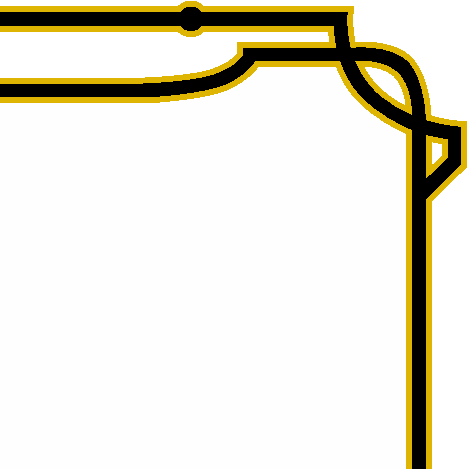
\includegraphics[width=\hbTableBorderS,height=\hbTableBorderS]{assets/fancy-table-corner}}
    \end{textblock*}%
    \begin{textblock*}{\linewidth}(\hbTableBoxWidth-\hbTableBorderS+\hbTableBorderX,\hbTableBoxHeight+\hbTableBoxDepth-\hbTableBorderS+\hbTableBorderY)%
    \scalebox{1}[-1]{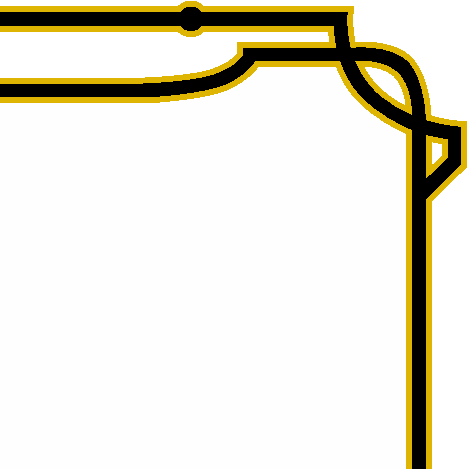
\includegraphics[width=\hbTableBorderS,height=\hbTableBorderS]{assets/fancy-table-corner}}
    \end{textblock*}%
    \begin{textblock*}{\linewidth}(-\hbTableBorderX+\hbTableBorderS,-\hbTableBorderY)%
    \scalebox{1}[1]{
\includegraphics[height=\hbTableBorderS,width=\hbTableBoxWidth-2\hbTableBorderS+2\hbTableBorderX]{assets/fancy-table-vert}}
    \end{textblock*}%
    \begin{textblock*}{\linewidth}(-\hbTableBorderX+\hbTableBorderS,\hbTableBoxHeight+\hbTableBoxDepth-\hbTableBorderS+\hbTableBorderY)%
    \scalebox{1}[-1]{
\includegraphics[height=\hbTableBorderS,width=\hbTableBoxWidth-2\hbTableBorderS+2\hbTableBorderX]{assets/fancy-table-vert}}
    \end{textblock*}%
    \begin{textblock*}{\linewidth}(-\hbTableBorderX,-\hbTableBorderY+\hbTableBorderS)%
    \scalebox{-1}[1]{
\includegraphics[height=\hbTableBoxHeight+\hbTableBoxDepth-2\hbTableBorderS+2\hbTableBorderY,width=\hbTableBorderS]{assets/fancy-table-horiz}}
    \end{textblock*}%
    \begin{textblock*}{\linewidth}(\hbTableBoxWidth-\hbTableBorderS+\hbTableBorderX,-\hbTableBorderY+\hbTableBorderS)%
    \scalebox{1}[1]{
\includegraphics[height=\hbTableBoxHeight+\hbTableBoxDepth-2\hbTableBorderS+2\hbTableBorderY,width=\hbTableBorderS]{assets/fancy-table-horiz}}
    \end{textblock*}%
    \usebox{\hbTableBox}\vspace*{\hbTableBorderY}%
    \TPoptions{absolute=true}%
}

\NewEnviron{hbNakedTable}[1]{%
  \hbTableBefore%
  \medbreak\noindent\begin{tabularx}{\linewidth}{#1}\BODY\end{tabularx}\medbreak%
}

\NewEnviron{hbNarrowTable}[3][h]{%
  \begin{table}[#1]%
    \caption{#2}%
    \hbTableBefore%
    \noindent\begin{tabularx}{\linewidth}{#3}\BODY\end{tabularx}%
  \end{table}%
}

\NewEnviron{hbWideTable}[3][t]{%
  \begin{table*}[#1]%
    \caption{#2}%
    \hbTableBefore%
    \noindent\begin{tabularx}{\linewidth}{#3}\BODY\end{tabularx}%
  \end{table*}%
}

\NewEnviron{hbFancyTable}[3][h]{%
  \begin{table}[#1]%
    \hbTableBefore%
    \sbox{\hbTableBox}{\colorbox{white}{\begin{minipage}{\linewidth-2\fboxsep}%
    \caption{#2}%
    \begin{tabularx}{\linewidth}{#3}\BODY\end{tabularx}%
    \end{minipage}}}%
    \hbTableDrawFancy%
  \end{table}%
}

\NewEnviron{hbFancyWideTable}[3][t]{%
  \begin{table*}[#1]%
    \hbTableBefore%
    \sbox{\hbTableBox}{\colorbox{white}{\begin{minipage}{\linewidth-2\fboxsep}%
    \caption{#2}%
    \begin{tabularx}{\linewidth}{#3}\BODY\end{tabularx}%
    \end{minipage}}}%
    \hbTableDrawFancy%
  \end{table*}%
}

%!TEX TS-program = xelatex
%!TEX encoding = UTF-8 Unicode

% Author: Romain "Artefact2" Dal Maso <artefact2@gmail.com>
% 
% This program is free software. It comes without any warranty, to the
% extent permitted by applicable law. You can redistribute it and/or
% modify it under the terms of the Do What The Fuck You Want To Public
% License, Version 2, as published by Sam Hocevar. See
% http://sam.zoy.org/wtfpl/COPYING for more details.

\newlength{\hbArtRealWidth}
\newlength{\hbArtFakeWidth}
\newlength{\hbArtRealHeight}
\newlength{\hbArtFakeHeight}
\newlength{\hbArtFakeHeightHack}

% XXX why the 1pt offset?
\newlength{\hbArtLeftOffset}
\setlength{\hbArtLeftOffset}{\maxof{\foremargin}{\spinemargin}+1pt}
\newlength{\hbArtOvershootWidth}
\setlength{\hbArtOvershootWidth}{\maxof{\foremargin}{\spinemargin}-\minof{\foremargin}{\spinemargin}+2pt}
\newlength{\hbArtTopOffset}
\setlength{\hbArtTopOffset}{\uppermargin}
\newlength{\hbArtBottomOffset}
\setlength{\hbArtBottomOffset}{\paperheight-\uppermargin-\textheight}

% XXX is it wise to use floats for this? they have a LOT of issues. Is
% it possible to alter the margins of the CURRENT page?  Look into
% geometry (inserts \clearpage, not good) and/or changepage (works but
% can't get it to reset the margins on next page automatically)

% XXX: left margin is wrong half the time, we need to overshoot

% W/H ratio, bottom spill fraction, Filename
\newcommand*{\hbWideBottomArt}[3]{%
  \FPeval{\result}{1/#1}%
  \setlength{\hbArtRealHeight}{\result\paperwidth}%
  \setlength{\hbArtFakeHeight}{#2\hbArtRealHeight}%
  \begin{figure*}[!b]%
    % XXX 1pt offset?
    \begin{rtb*}{\paperwidth+\hbArtOvershootWidth}{-\hbArtLeftOffset}{\hbArtFakeHeight-\hbArtRealHeight}%
      \includegraphics[width=\paperwidth+\hbArtOvershootWidth,height=\hbArtRealHeight]{#3}
    \end{rtb*}%
    \rule{0pt}{\maxof{0pt}{\hbArtFakeHeight-\hbArtBottomOffset}}%
  \end{figure*}%
}

\newcommand*{\hbWideTopArt}[3]{%
  \FPeval{\result}{1/#1}%
  \setlength{\hbArtRealHeight}{\result\paperwidth}%
  \setlength{\hbArtFakeHeight}{#2\hbArtRealHeight}%
  \begin{figure*}[!t]%
    \begin{rtb*}{\paperwidth+\hbArtOvershootWidth}{-\hbArtLeftOffset}{-\hbArtTopOffset}%
      \includegraphics[width=\paperwidth+\hbArtOvershootWidth,height=\hbArtRealHeight]{#3}
    \end{rtb*}%
    \rule{0pt}{\maxof{0pt}{\hbArtFakeHeight-\hbArtTopOffset}}%
  \end{figure*}%
}

% XXX: https://tug.org/TUGboat/tb35-3/tb111beet-banner.pdf
% It's ugly and limited, but also the best TeX can do
\newcommand*{\hbWideBottomArtFirstPageFix}{}
\newcommand*{\hbWideBottomArtFirstPage}[3]{%
  \FPeval{\result}{1/#1}%
  \setlength{\hbArtRealHeight}{\result\paperwidth}%
  \setlength{\hbArtFakeHeight}{#2\hbArtRealHeight}%
  \setlength{\hbArtFakeHeightHack}{\maxof{0pt}{\hbArtFakeHeight-\hbArtBottomOffset}}%
  \renewcommand*{\hbWideBottomArtFirstPageFix}{\enlargethispage{-\hbArtFakeHeightHack}}%
  \begin{figure}[!b]%
    \begin{rtb*}{\paperwidth+\hbArtOvershootWidth}{-\hbArtLeftOffset}{\hbArtFakeHeight-\hbArtRealHeight}%
      \includegraphics[width=\paperwidth+\hbArtOvershootWidth,height=\hbArtRealHeight]{#3}
    \end{rtb*}%
    \rule{0pt}{\hbArtFakeHeightHack}%
  \end{figure}%
}

\newcommand*{\hbFullPageArtHook}[1]{%
  \AddThispageHook{%
    \begin{tb*}{\paperwidth}{0pt}{0pt}%
      \includegraphics[width=\paperwidth,height=\paperheight]{#1}
    \end{tb*}%
    \begin{tb*}{\paperwidth}{0pt}{0pt}%
      
\includegraphics[width=\paperwidth,height=\paperheight]{assets/full-page-decoration}
    \end{tb*}%
  }%
}

\newcommand*{\hbFullPageArt}[1]{%
  \clearpage\hbFullPageArtHook{#1}\null\clearpage%
}

\newcommand*{\hbFloatArt}[2][h]{%
\begin{figure}[#1]%
\centering%
\includegraphics[width=.8\linewidth]{#2}%
\end{figure}%
}

% W/H, x-spill, y-spill, x-offset, y-offset, rule-height, floatspec, filename
\newcommand*{\hbArtCornerInternal}[8]{%
\setlength{\hbArtFakeWidth}{\linewidth+\hbArtLeftOffset}%
\FPeval{\result}{1/#3}%
\setlength{\hbArtRealWidth}{\result\hbArtFakeWidth}%
\FPeval{\result}{1/#1}%
\setlength{\hbArtRealHeight}{\result\hbArtRealWidth}%
\setlength{\hbArtFakeHeight}{#2\hbArtRealHeight}%
\begin{figure}[#7]%
\begin{rtb*}{\hbArtRealWidth}{#4}{#5}%
\includegraphics[width=\hbArtRealWidth]{#8}
\end{rtb*}%
\rule{0pt}{\maxof{0pt}{#6}}%
\end{figure}%
}

% W/H, top spill, right spill, filename
\newcommand*{\hbBottomLeftArt}[4]{%
\hbArtCornerInternal{#1}{#2}{#3}{-\hbArtLeftOffset}{\hbArtFakeHeight-\hbArtRealHeight}{\hbArtFakeHeight-\hbArtBottomOffset}{!b}{#4}%
}

% W/H, top spill, left spill, filename
\newcommand*{\hbBottomRightArt}[4]{%
\hbArtCornerInternal{#1}{#2}{#3}{\hbArtFakeWidth-\hbArtRealWidth}{\hbArtFakeHeight-\hbArtRealHeight}{\hbArtFakeHeight-\hbArtBottomOffset}{!b}{#4}%
}

% W/H, bottom spill, right spill, filename
\newcommand*{\hbTopLeftArt}[4]{
\hbArtCornerInternal{#1}{#2}{#3}{-\hbArtLeftOffset}{-\hbArtTopOffset}{\hbArtFakeHeight-\hbArtTopOffset}{!t}{#4}%
}


% W/H, bottom spill, left spell, filename
\newcommand*{\hbTopRightArt}[4]{%
\hbArtCornerInternal{#1}{#2}{#3}{\hbArtFakeWidth-\hbArtRealWidth}{-\hbArtTopOffset}{\hbArtFakeHeight-\hbArtTopOffset}{!t}{#4}%
}


\newcommand*{\hbLettrine}[2]{\lettrine[lines=6,nindent=0pt]{{\solberaimitation #1}}{#2}}
\newcommand*{\hbLettrined}[2]{\lettrine[lines=6,depth=1,nindent=0pt]{{\solberaimitation #1}}{#2}}
\renewcommand*{\LettrineTextFont}{\mreaves}

\newcommand*{\hbNone}{\rule[0.2\baselineskip]{1em}{.75pt}}

% StrokeColor, FillColor, StrokeWidth, Text
\newcommand*{\fillstroke}[4]{%
% this is black magic
% ref: http://tex.stackexchange.com/a/225639/125447
% Tr: rendering mode (0=Fill, 1=Stroke, 2=FillThenStroke)
% w: stroke width
\special{pdf:bcolor #1 #2}%
\special{pdf:literal direct #3 w 2 Tr}%
#4%
% ref: http://project.ktug.org/dvipdfmx/doc/tug2005.pdf
\special{pdf:ecolor}%
\special{pdf:literal direct 0 Tr}%
}

\usepackage{bbding}
\usepackage{ifthen} % to omit tables in the monsters section from the lot
\usepackage[noautomatic]{imakeidx}
\makeindex[columns=1, title=Monsters Alphabetically]
\indexsetup{level=\hbRootAppendix,firstpagestyle=hbRegular}
\twocolumn
\sloppy
\setlength{\parindent}{1em}

% The PHB isn't justified. In my opinion, raggedright looks worse, to
% disable it comment these two lines.
%\raggedright % Messes up the indent.
%\setlength{\parindent}{1em}

% Uncomment for white background (for print)
%\renewcommand{\hbBackground}{assets/background-print}

\newcommand{\DND}{\emph{Dungeons \& Dragons}}
\newcommand{\PHB}{\emph{Player's Handbook}}
\newcommand{\DMG}{\emph{Dungeon Master's Guide}}
\newcommand{\MH}{\emph{Monster Hunter}}

\newcommand{\imageheader}[3]{%
\vspace{10pt plus 10pt minus 2pt}%
\noindent\begin{minipage}[c]{1cm}%
\includegraphics[width=\linewidth]{#1.png}%
\end{minipage}\hspace{1em}%
\begin{minipage}{0.8\linewidth}%
\subsubsection*{#2}%
{\itshape #3\par}%
\end{minipage}\nopagebreak\\[3pt]\nopagebreak}

\newcommand{\monsterheader}[4]{%
\vspace{10pt plus 10pt minus 2pt}%
\noindent\begin{minipage}[c]{1cm}%
\includegraphics[width=\linewidth]{#1.png}%
\end{minipage}\hfill%
\begin{minipage}{\dimexpr -1em-1cm+\linewidth}%
\subsection*{#2}\index{#2}%
{\textit{Rating: } \raisebox{-2pt}[0pt]{#3} \textit{(#4)}\par}%
\end{minipage}\nopagebreak\\*[3pt]}

\newcommand{\smallicon}[1]{\raisebox{-2pt}[0pt]{\includegraphics[height=\baselineskip]{#1}}}
\newcommand{\tableicon}[1]{\smallicon{assets/ext/icons/#1}}
\newcommand{\sizecrowns}[2]{\hfill\mbox{\footnotesize\tableicon{crown-small}\,#1\,cm\quad\tableicon{crown-gold}\,#2\,cm\par}}

\begin{document}

\frontmatter

\renewcommand{\hbTitle}{Monster Hunter \protect\\ in D\&D 5e}
\renewcommand{\hbSubtitle}{Created by Scaatis, using \texttt{texbrew}\protect\\ \url{https://github.com/Artefact2/texbrew/}}
\renewcommand*{\hbCover}{assets/ext/classic}
\hbMakecover

% Use assets/background if you don't want a cover. You can put your
% own assets under assets/ext/.
\renewcommand*{\hbSubcover}{assets/ext/classic2}
\hbMakesubcover

%\paragraph*{Acknowledgments} {\footnotesize \lipsum[100-101]}

\paragraph*{Credits}

{\footnotesize
\begin{itemize}
\item D\&D, the D\&D logos are intellectual property of Wizards of the
  Coast LLC.

\item Some decorations (footers, headers, etc.) were ripped and
  vectorialised from the Player's Handbook and are probably not safe
  to redistribute as such.

\item The fonts in this documents were made by Reddit user /u/Solbera,
  and are released under the CC-BY-SA 4.0 license.

  \url{https://www.reddit.com/r/UnearthedArcana/comments/3vpphx/5e_font_package_embeddable_cc_edition/}

\item The background image is from the Homebrewery, created by Scott
  Tolksdorf, and is released under the MIT license.

  \url{https://github.com/stolksdorf/homebrewery}

\item This book template was created by Romain ``Artefact2'' Dal Maso,
  and was typeset using \XeTeX.

  \url{https://artefact2.com/}

  \url{https://github.com/Artefact2/texbrew/}
      
  \url{http://xetex.sourceforge.net/}

%\item Monster Hunter copyright CAPCOM and all that
\item Lots of information from the Monster hunter wiki

\url{http://monsterhunter.wikia.com}

\item The fine gentleman (or lady) from the MHLore tumblr

\url{http://mhlore.tumblr.com/}

\item Image Credits: \begin{itemize}

\item ``Guildmarm'' by Ming-Yin Wong

\url{https://lagunis.artstation.com/projects/rJER5}
\item ``Sojourn'' by DeviantArt user arvalis

\url{http://arvalis.deviantart.com/art/Sojourn-205826444}

\item ``溪流'' by Yu Yiming

\url{https://www.artstation.com/artwork/xBJ02}

\item ``Field of Gold'' by DeviantArt user Hangmoon

\url{http://hangmoon.deviantart.com/art/Fields-of-gold-492963608}

\item ``Mountain Path'' by DeviantArt user UnidColor

\url{http://unidcolor.deviantart.com/art/Mountain-Path-126000708}

\item ``Dangerous Hunt'' by Phil Dragash

\url{https://www.artstation.com/artwork/A4yDo}

\item ``Lagiacrus Fan Illustration'' by Selicato Mattia

\url{https://www.artstation.com/artwork/gyRGZ}

\item ``Forest Sleeps'' by Kullen MacFarlane

\url{http://endivinity.artstation.com/projects/gVaDE}

\item ``Chameleos Fanart'' by Lucas Damon

\url{https://www.artstation.com/artwork/monster-hunter-fan-art-chameleos}
\end{itemize}
 % You can probably omit this if you don't use any of the sample assets
\item Monster Hunter copyright CAPCOM and all that
\item Lots of information from the Monster hunter wiki

\url{http://monsterhunter.wikia.com}

\item The fine gentleman (or lady) from the MHLore tumblr

\url{http://mhlore.tumblr.com/}

\item Image Credits: \begin{itemize}

\item ``Guildmarm'' by Ming-Yin Wong

\url{https://lagunis.artstation.com/projects/rJER5}
\item ``Sojourn'' by DeviantArt user arvalis

\url{http://arvalis.deviantart.com/art/Sojourn-205826444}

\item ``溪流'' by Yu Yiming

\url{https://www.artstation.com/artwork/xBJ02}

\item ``Field of Gold'' by DeviantArt user Hangmoon

\url{http://hangmoon.deviantart.com/art/Fields-of-gold-492963608}

\item ``Mountain Path'' by DeviantArt user UnidColor

\url{http://unidcolor.deviantart.com/art/Mountain-Path-126000708}

\item ``Dangerous Hunt'' by Phil Dragash

\url{https://www.artstation.com/artwork/A4yDo}

\item ``Lagiacrus Fan Illustration'' by Selicato Mattia

\url{https://www.artstation.com/artwork/gyRGZ}

\item ``Forest Sleeps'' by Kullen MacFarlane

\url{http://endivinity.artstation.com/projects/gVaDE}

\item ``Chameleos Fanart'' by Lucas Damon

\url{https://www.artstation.com/artwork/monster-hunter-fan-art-chameleos}
\end{itemize}

\end{itemize}}

\clearpage
\tableofcontents*

\vfill\break
\listoftables*

\mainmatter

\hbRootChapter{Introduction}

\hbBottomLeftArt{.751}{.95}{.85}{assets/ext/guildmarm-corner}

\hbLettrine{W}{elcome, Hunter,} to the world of Monster Hunter! It is a wide open, sparsely populated land full of lush landscapes teeming with wildlife, for better or worse. Large cities are rare, you will find the small village nestled in a protected niche to be far more common. The world is a wild and dangerous place, teeming with monsters and ancient secrets.

\begin{hbNote}[t]
\subsubsection*{What does he know?}
\noindent As with any supplement, feel free to ignore anything and everything written here and have your setting work how you want it to. Hell, I don't follow half the advice in this book.
\end{hbNote}

Hunters deal with the monster population, but there are many more adventures to be found out in the wilderness. The few large cities are true marvels of the world, protected by ingenious defensive structures such as the battlequarters of Dundorma. The resourcefulness of the cities' engineers allows these few bastions to stand against the wild monsters and the far more devious dragons.

While I have tried to stick with the \MH{} Canon as much as possible, there is not a great deal of detail we get from the games themselves. I have filled in gaps in many places and added my own details. From the games we get a much better impression of the \emph{feeling} of the world rather than the exact details of the setting.

The feeling is this: The world is vast and alive, vibrant and colorful. It is nature at its most savage, and yet its inhabitants live in the moment and enjoy it, rather than fearing for tomorrow. Don't worry about getting the location of Dundorma wrong in your game. It is far more important to convey the feeling of the lush forests and endless plains, of something always lurking behind the next bush, on the prowl. The world is dangerous. The ladder of monsters \emph{starts} with velociraptors and goes all the way up to world eating dragons of the ancient times.

\subsection{Adaptation Pains}
\MH{} wasn't made with \DND{} in mind, so it is not surprising that some assumptions of the two systems don't match up. Here are some aspects that need adaptation and my take on how to reconcile them:

\subsubsection{Magic}
In the \MH{} canon, there are no spellcasters. There are certainly no hunters who primarily use magic to fight. Taking magic out of \DND{} takes too much out of the experience in my opinion. If you and your group don't want to use magic, don't. Here are some thoughts on it regardless:
\begin{itemize}
\item Magic users are rare. There are no institutions to learn magic, such as a magical college. An attempt to establish such a thing could be a campaign in its own right.
\item A wizard character would have learned his art directly at the hand of a master and might be expected to take an apprentice when he is experienced enough.
\item Spells that raise the dead or travel between planes are not learned normally. They may exist, but special measures must be taken to learn them.
\item Some (but not all) magic relates to spirits (see above). Perhaps instead of summoning an earth elemental, consider flavouring it as an earth spirit. When creating a flaming sword, one creates the sword and prepares it in such a way as to be a vessel for a fire spirit to inhabit. This provides an interesting explanation for why your sword \textit{must} be so richly decorated: It must provide a pleasing vessel for the spirit to come willingly. A more evil mage might bind a spirit to the sword against its will.
\item In addition to spellcasting magic, there is the field of alchemy. This need not have anything to do with the occult, but simply be a craft that exploits the special properties of the herbs or monster parts to make potions of seemingly magical effect. Or it could be magic.
\end{itemize}

\subsubsection{Religion}

\hbWideBottomArtFirstPage{1.784}{.892}{assets/ext/sojourn}

Be it clerical magic or literal divine intervention, the gods play an important role in \DND. The people in the Monster Hunter games don't typically make references to a god or gods, except when referring to certain monsters (mostly Elder Dragons). There might be people who see the Elder Dragons as gods, but no sane person would worship them. It is conceivable, however, that in some areas, people make sacrifices to avert the threat of an Elder Dragon attack. One could see the dragons as living creatures of legend, but some imbue them with divinity, which makes them a natural force and an integral part of the universe. That raises some question about the consequences of hunting them\ldots

As far as mainstream religion is concerned, the games do make references to spirits at times. I would suggest using the rules for spiritualism from the \DMG. I won't reproduce the text here, but essentially it describes the belief that everything is inhabited by a spirit. One doesn't worship one particular spirit but instead reveres and respects them all. A clerical domain represents a spirit who is particularly close to you, whom you might even know personally and whose powers you are able to wield specifically. Otherwise, you channel the powers of the combined spirit world. That means you are free to chose whatever cleric domain you wish.

\subsubsection{Miscellaneous}
Some short notes that didn't warrant their own categories:

\paragraph{Falling Damage.} There is no falling damage in \MH{}. Neither for players nor for Monsters. Let's see you abuse that.
\paragraph{Sand.} Sand is basically water for monsters that can swim in it. Given the right items, the players might be able to swim in it as well, but otherwise, it's solid ground for them and water for the monsters.
\paragraph{Holding Your Breath.} In \MH{}, everyone is Guybrush Threepwood and can hold their breath for ten minutes. I would go so far as to say everyone can just breathe underwater and save myself the bookkeeping.
\paragraph{Video Game Flair.} \MH{} is pretty comical. In a lot of places, I kept using the video game mechanics pretty much unchanged, usually to comedic effect, such as the falling damage. One other example would be additional drops from getting breaks on monster parts. It's very videogamey (why do I get the King's Frills from Great Jaggi if I \emph{break} the frills?) but it fulfills the same purpose it does for the video game: It rewards going for those risky breaks and getting the rare drop is sweet.
\hbWideBottomArtFirstPageFix


%\begin{figure}[b!]
%%\includegraphics[width=\linewidth]{Guildmarm}
%\end{figure}

\renewcommand*{\hbPartCover}{assets/ext/world-cover}
\renewcommand*{\hbPartSubcover}{assets/ext/world-cover2}

\part{Exploring the World}

\chapter{Geography}

\hbWideBottomArtFirstPage{1.784}{.892}{assets/ext/fields-of-gold}

Though population is sparse, life flourishes in every corner of the world. People have constructed impressive cities despite the constant threat of monster attack everywhere from the scorching desert to freezing mountaintops. And in between the buildings of the modern civilisation we can find the ruins of those who came before us, a mysterious society only known as the Ancient Civilisation.

\section{Regions}
We are not given an estimate of the size of the Monster Hunter World. The size of the world is an important customisation factor. We know that the Hunter's Guild is a single global organisation. While its administration is decentralised this still implies that one can travel from one end to the continent in reasonable time. But how long is reasonable? Without a forced march, characters can travel 30 miles per day at fast pace (a reckless act considering how dangerous the world is). These are various options for the size of your world:

\paragraph{Small} Minegarde and Dundorma are about 600 miles apart, or 20 days of travel (about the distance of Berlin to Paris). That puts the total coast to coast distance of the continent to about 1500 miles or 50 days of travel.

\paragraph{Medium} Minegarde and Dundorma are about 1500 miles apart (about the distance between London and Moscow). The whole continent is 3800 miles (about 130 days of travel) east to west.

\paragraph{Large} The continents on the map, which somewhat resemble Europe, Asia and Africa are about the same size as those real-life continents. That means the width of the main continent are about 6000 miles, or 200 days of fast travel pace. Dundorma and Minegarde are about 2400 miles apart.

\hbWideBottomArtFirstPageFix

\begin{hbNoteWide2}[b]
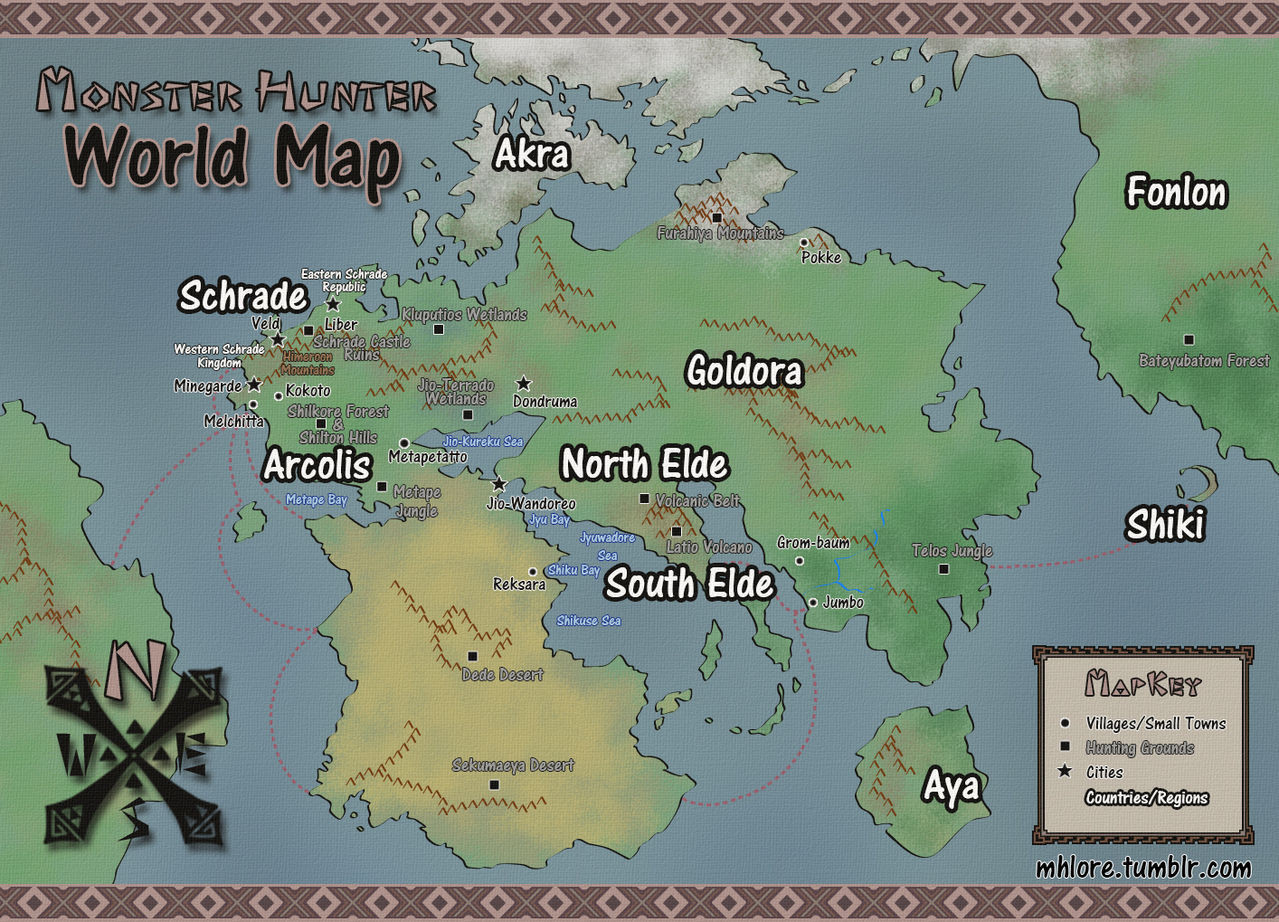
\includegraphics[width=\textwidth]{assets/ext/MHMap.jpg}
\end{hbNoteWide2}

\subsection*{Schrade}
This region was split in two by a civil war long ago, and is now divided into the Western Schrade Kingdom and the Eastern Schrade Republic, with the ancient ruins of Castle Schrade positioned roughly in the middle.

\paragraph{Liber} The capital of the Eastern Schrade Republic. Situated in a basin surrounded by steep mountains, it is subjected to severe weather and long winters. It is a prosperous and egalitarian trade city, famous for its monster hunting caravans. The center of town is dominated by a heavily fortified tower for monitoring and repelling large monsters.

\paragraph{Veld} The capital of the Western Schrade Kingdom. A walled fortress city of opulent aristocrats. The poor are relegated to slums outside the city walls, an area sarcastically named "The Painting District".

\paragraph{Castle Schrade} An ancient castle located in the vast open plain in the center of Schrade. Once a splendid feudal manor, it is now a mere shadow of its former glory, surrounded only by the ruins of the villages and towns that used to encircle it. So complete is the devastation, that no one remains to mourn its passing.

\paragraph{Kokoto Village} A small town of subsistence farmers in a forested area with a mild climate. The village relies on its chief and his deep understanding of monsters and monster ecology to maintain a peaceful relationship with nearby monsters, however, hunters are still needed on occasion to defend the town.

\paragraph{Minegarde} The city of Minegarde is an outpost built on a small outcropping with several caves among the rocky cliffs.  It was found to be rather unsuitable for usual human habitation due to the arid, rocky location and large amounts of dangerous monsters, so it became a haven for hunters and those that do business with them.  Because of the monsters, Minegarde also has multiple cannons for defense.  The cave that the blacksmith is located in is used as an emergency shelter for the locals should monsters attack.  The blacksmiths of Minegarde are also responsible for creating the first prototypes for the Gunlance.

\subsection*{Arcolis}
\paragraph{Melchitta} Melchitta is a rather new village situated on the shore of The Great Circle Lake, a lake that was formed by a meteor strike. It was originally just a tiny hunting village until some scholars from Minegarde took note of it, and now trade is booming.

\paragraph{Loc Lac} Loc Lac is a large, prosperous desert city built at the edge of the sand sea, near a large lake. The lake was formed when Jhen Mohran crashed into the rocks and its tusk lodged into the earth so deeply it struck water. The people of Loc Lac consider Jhen to be a symbol of prosperity, because the creation of the lake allowed the city to flourish. They hold the "Festival of Fear" every time the sandstorms arrive that herald Jhen's approach.

\subsection*{Akra}
Far to the North is the freezing, ice-covered Akra Region, known for its volatile weather. Despite the harsh conditions, it is surprisingly well populated. However, no major cities are located there.

\subsection*{Aya}
Far to the south is the island nation of Aya. It boasts a multitude of extremely varied tribal cultures, which a single absolute monarchy has (attempted) to rule over for generations.  Although most of the land's cultures are extremely isolationist, even those that aren't are still shrouded in mystery.

\subsection*{Fonlon}
\paragraph{Bateyubatom Forest} Also known as the Great Forest or the Everwood, this forest is home to a great variety of monsters and was also a major site of the old civilisation, as evidenced by the many ruins found scattered around the region.

\subsection*{Dundorma} Dundorma is located smack in the middle of the main continent, just on the other side of the Himeroon mountains. Due to its location it is constantly under threat from monsters, especially Elder Dragons. Despite having been destroyed repeatedly, it is always rebuilt and reinforced. As a result, its population fluctuates somewhat, but it is considered the largest city in the world with about 20,000 inhabitants. Dundorma is the seat of the Hunter's Guild administration, as well as the home of His Immenseness, the Great elder of Dundorma, a wise old wyverian respected all across the world.

\noindent\textit{Note: The name is sometimes given as Dondruma. This is because the translators decided to change the name in MH4U to Dundorma to more closely match the Japanese pronunciation. Before that, the town was named Dondruma.}

\subsection*{North Elde}
This northern stretch of the volcanic peninsula is actually under the jurisdiction of the Minegarde division of the Hunter's Guild.  Near the hunting grounds is a thriving smithing village named N'ganga, which hunters often use as a base when hunting and mining in the area.  It is unmarked on the map.

\hbBottomLeftArt{.751}{.95}{.85}{assets/ext/mountain-sketch}

\paragraph{Harth} Harth is the home of the Troverians, an industrious race of dwarf-like folk who mine the local volcano and use its magma to power their forges.

\subsection*{South Elde}
The southern end of the peninsula is under Dondruma's jurisdiction.  Similarly to North Elde, there is another unmarked town, a fishing village, on the southern tip which often does trade with surrounding villages like Jumbo.

\subsection*{Goldora}
\paragraph{Tanzia} Tanzia Port is a bustling port located on a rocky cliffside in a tropical area, famous for its giant lighthouse and the delicious food of the felyne-owned-and-run Tanzinya Grill.

\paragraph{Pokke Village} The Furahiya Mountain Range has been wrapped in snow since ancient times, never seeing a single thaw. Known for its Ice Crystals and Mountain Herbs, the Furahiya range is also home to Pokke Village. At the center of the village, and its most well known feature, is a huge stone made of Machalite Ore. A piece of ore this large is extremely rare. This piece of Machalite was what attracted a brother and sister pair of Wyverians to open up a path and start this village. This village was founded hundreds of years ago. With the abundance of Machalite lines near the village, it became an incredibly prosperous mining village. In modern Pokke, a hot spring shoots from the center of the peaceful village. Other than mining, it is home to hunters seeking fame and fortune in the Snowy Mountains, and tourists seeking rejuvenation in the hot springs.

\paragraph{Jumbo Village} A trade port on the coast. Originally a run-down and beleaguered little village, it was renovated and turned into a prosperous town by the Jumbo Village Chief.

\subsection*{Shiki}
\paragraph{Cathar} Cathar is an isolated Wyverian farming village high on a wind-swept plateau near Heaven's Mount. The wyverians here are unusually superstitious and spiritual.  The village's Japanese name, Shinato, is a reference to Shinato no Kaze, the purifying wind.

%\hbFullPageArt{assets/ext/mountain-path}

\chapter{The Peoples of the World}

The world is inhabited primarily by three species of humanoids: Humans, wyverians and lynians. Wyverians are tall and hardy, with parts of their bodies protected by scales. Lynians are small and nimble and often live seperate from society of humans and wyverians.

In addition to these three major species, there are a great number of minor species, often living only in one particular place, such as the dwarf-like troverians or the fish people of Jumbo Village. If the races provided here are not to your taste, you are encouraged to develop your own.

\hbWideBottomArtFirstPage{1.784}{.892}{assets/ext/palicoes}

\subsection*{Names}
Most characters in in \MH{} don't have names, but are referred to by monikers or job description. One smith calls himself The Man and the village chief is simply called Village Chief. Monikers can work, but job descriptions can get confusing if you know multiple Village Chiefs. You can choose to follow with this guideline from the games or choose names like you would normally. A major exception to this rule are palicoes, which have a variety of cat names.

\section{Lynians}
Lynians are small, bipedal creatures with tribal, often primitive societies.  While they often live in communities of their own, there are often individuals living with humans and wyverians.

\subsection*{Lynian Traits}
\paragraph{Ability Score Increase.} Your Dexterity score increases by 2.

\paragraph{Age.} Lynians live much shorter lives than humans do, maturing at the age of 3, and live to about 15.

\paragraph{Alignment.} Felynes tend to be good, Melynx neutral and Shakalaka evil. They all value and admire bravery above all, whether it is bravery to protect one's people, bravery to prove oneself over others or bravery to crush all foes.

\paragraph{Size.} Lynians are about 3 feet tall and weigh 40 pounds. Your size is Small.
\hbWideBottomArtFirstPageFix

\paragraph{Speed.} Your base walking speed is 25 feet.

\paragraph{Nine Lives.} You only die after failing four death saving throws, rather than three.

\paragraph{Darkvision.} You have superior vision in dark and dim conditions. You can see in dim light within 60 feet of you as if it were bright light, and in darkness as if it were dim light. You can't discern color in darkness, only shades of gray.

\paragraph{Lynian Nimbleness.} You can move through the space of any creature that is larger than you.

\paragraph{Weapon Proficiency.} You are proficient with the Felyne Catspaw.

\paragraph{Languages.} You speak Felyne and one other language (usually Common). Other races have difficulty mimicking the cat sounds that make up the Felyne language, so not many non-Lynians speak it.

\paragraph{Subrace.} There are two playable Lynian subraces, Felyne and Melynx.

%\subsubsection*{Felyne}
\imageheader{assets/ext/icons/Felyne}{Felyne}{}

Felynes are the most well-known of the lynians.  They are small cat-like people, typically beige in color with brown markings, although a rainbow of colors and a variety of markings are possible. In the wild, they live in small villages with their close cousins the melynx. They do not appear to have written language, but they do pass down tales and stories orally, and they do paint pictograms and symbols onto rocks and other surfaces to mark and decorate their homes. While they are not great builders and architects, their cat-shaped houses are richly painted and beautiful in their own way.

Their villages can be found literally everywhere, from frozen tundras to volcanic caves, as the felynes themselves are extremely hardy and resourceful. They tend to burrow into the sides of cliffs to make their dens, although they are capable of constructing buildings with wood, thatch, clay, and other found materials.

Of the lynians, they are the most integrated into human and wyverian society. They usually take on service or labour jobs such as cooking and cleaning, selling items, or working as farm hands or blacksmith's assistants. This may be because they genuinely enjoy this work, or because they are discriminated against by society. Of course, the most dangerous and most glorified profession for them is that of palico, being hunting companions for human and wyverian monster hunters. The Hunter's Guild does not recognize palicoes as hunters in their own right, but that hardly bothers the palicoes. As far as they are concerned, they are not second fiddle to hunter, the hunter is privileged to accompany \textit{them} on their glorious adventures.

When playing a felyne or melynx, consider using as many cat-related puns as possible, until your group threatens you with physical violence. Then use even more.

Felynes admire bravery above all else and a successful palico enjoys a high standing in their society. They also recognize the need for wisdom, so one often finds an old wyverian living out his days among palicoes, much like they do in human society, providing advice and guidance to the tribe.

\paragraph{Ability Score Increase.} Your Constitution score increases by 1.

\paragraph{Brave.} You have advantage on saving throws against fear.

\paragraph{Blind Luck.} Whenever you roll a 1 on a saving throw, you may reroll the die and must use the new roll.

%\subsubsection*{Melynx}
\imageheader{assets/ext/icons/Melynx}{Melynx}{}

%\begin{figure}\begin{center}\includegraphics[width=0.6\linewidth]{MelynxRender.png}\end{center}\end{figure}

Melynx are the close cousins of felynes, and are noted for their black and white fur with black and pink markings, although other shades exist among melynx palicoes.  They wear handkerchiefs and pouches made of woven green grasses, and carry their cat paw staves. Melynx are known for their thievery, as hunters are well aware of their tendency to attack and steal items without provocation while out in the field.  Because of this, they're often labeled kleptomaniacs, and are far less tolerated in human and wyverian society than felynes are.

The truth is probably more complicated than that. Felynes and melynx live together in their villages, often in harsh environments where they may be forced to steal to survive. Why this job is mostly done by the melynx is not known.

\paragraph{Ability Score Increase.} Your Charisma score increases by 1.

\paragraph{Naturally Stealthy.} You can attempt to hide even when you are obscured only by a creature that is at least one size larger than you.

\paragraph{Catlike grace.} You are proficient with the Acrobatics skill.

\subsubsection*{Shakalaka}

%\begin{figure}[b!]
%\centering
%\includegraphics[width=0.8\linewidth]{ShakalakaRender.png}
%\end{figure}

\hbBottomRightArt{1.252}{.95}{.85}{assets/ext/gathering-hall}

Shakalakas are the last group of lynians, and are more distantly related to felynes and melynx.  They are small, green-skinned, goblin-like creatures, known for always wearing masks and for their dancing. They are extremely aggressive, attacking hunters who wander too close, often by popping out of holes in the ground to ambush them.  They live in very primitive tribal societies, with little to no known architecture, or writing, (and no art aside from their masks.) Each tribe is headed by a larger King Shakalaka, who often wears a flaming barbecue spit for a crown and attacks by hurling fireballs and swinging wildly with his club (which is usually a haunch of meat).  Young shakalaka often change their masks, but upon entry to adulthood, go off on a quest to find the one mask that they will wear as an adult.

\section{Humans}

Humans are the second-most technologically advanced race in the Monster Hunter world, and are rather self-explanatory. They come in a variety of shapes, colors, and sizes, and are the most populous race in the MH world (well, more populous than wyverians, at any rate, it's unknown how they compare to lynians.) Humans founded the Hunter's Guild, the most important organization in their society.

\subsection*{Human Traits}
Humans use the same rules as in the \PHB.

%\begin{figure}[h]\includegraphics[width=\linewidth]{Humans.jpg}\end{figure}

\section{Troverians}

%\begin{figure}\includegraphics[width=\linewidth]{Troverians.png}\end{figure}

Troverians are an industrious dwarf-like people originating from Harth. Troverians are known to prefer living in underground areas, due to them using the many ores and minerals in the areas to produce equipment such as armour and weapons. The troverians seem to learn how to make such equipment from the wyverians. Some troverian tribes even have special ways to polish old equipment found in the field by hunters. This race is said to be "workaholics" due to them working for long periods. They can continue work day and night to produce such equipment without a need to sleep until their work is finished. Many of the troverian's clothes allow them to continue working without much problem, while also acting as their usual attire.

\subsection*{Trovierian Traits}
\paragraph{Abiltiy Score Increase.} Your Constitution score increases by 2 and Strength score increases by 1.

\paragraph{Age.} Troverians age in roughly the same way as humans do, reaching maturity in their teens and living to about 70.

\paragraph{Alignment.} Troverians care most of all about wanting to work. As such, they are usually neutral or chaotic good.

\paragraph{Size.} Troverians stand between 4 and 5 feet tall. Your size is Medium.

\paragraph{Speed.} Your base speed is 25 feet.

\paragraph{Darkvision.} Accustomed to life underground, you have superior vision in dark and dim conditions. You can see in dim light within 60 feet of you as if it were bright light, and in darkness as if it were dim light. You can't discern color in darkness, only shades of gray.

\paragraph{Troverian Resilience.} Troverians can go for up to four days without resting, though they do not gain the benefits of resting in that time.

\paragraph{Weapon Proficiencies.} You have proficiency with the Hammer, Lance and Gunlance.

\paragraph{Tool Proficiency.} You gain proficiency with the artisan's tools of your choice: smith's tools, brewer's supplies, or mason's tools.

\paragraph{Artisan's Cunning.} Whenever you make an Intelligence\,(History) check related to the origin of metalwork, you are considered proficient in the History skill and add double your proficiency bonus to the check, instead of your normal proficiency bonus.

\paragraph{Languages.} You know Common and Troverian. Troverian is a deep, melodic language with a humming sound.

\paragraph{Armor Proficiency.} You have proficiency with light and medium armor.

\hbTopRightArt{1.34}{1.0}{0.95}{assets/ext/troverians}

\section{Wyverians}

\hbWideTopArt{2.01}{.95}{assets/ext/azure-rathalos}

Wyverians have long pointed ears, 4 digits on their hands and feet, and have extremely long life-spans. All of this stems from the fact that they are evolved from wyverns, despite their rather human-ish appearance.  Some of them still have scales on their hands and feet, and have sharp, black, claw-like nails. Although most have light skin, wyverians with darker skin do exist. Wyverians are extremely variable in their appearance, even having some rather extreme differences in their anatomy.  Young wyverians tend to be roughly human-sized, while old wyverians tend to be very short, almost felyne-sized.

They are the most technologically advanced race in MH, as most tech in the world was either invented or at least improved upon by them. Their style of blacksmithing is so complex it is usually assumed to be impossible for other races to master it, thus the majority of blacksmiths in the world are wyverian. They are usually at the top of the social ladder, often having high-ranking positions, especially in the Guild, but can also be found as merchants and occasionally even monster hunters.

\subsection*{Wyverian Traits}
\paragraph{Ability Score Increase.} Your Intelligence score increases by 2 and your Constitution by 1.

\paragraph{Age.} Wyverians reach physical maturity around the same age as humans do, but define adulthood by experience, which can mean they reach adulthood anywhere between 40 and 100 years. They live for about 400 years.

\paragraph{Alignment.} Most Wyverians are lawful good.

\paragraph{Size.} Wyverians range from 5 to over 7 feet tall. Your size is Medium.

\paragraph{Speed.} Your base walking speed is 30 feet.

\paragraph{Darkvision.} You have superior vision in dark and dim conditions. You can see in dim light within 60 feet of you as if it were bright light, and in darkness as if it were dim light. You can't discern color in darkness, only shades of gray.

\paragraph{Keen Senses.} You have proficiency in the Perception skill.

\paragraph{Hard Skin.} Your armor class is increased by 1. This bonus stacks with worn armour.

\paragraph{Wyvern Ancestry.} You have advantage on saving throws against being charmed.

\paragraph{Languages.} You know Common, Wyverian and one other language of your choice. Wyverian is similar to Japanese.

\paragraph{Cantrip.} You know one cantrip of your choice from the wizard spell list. Intelligence is your spellcasting ability for it.

\paragraph{Weapon Proficiencies.} You have proficiency with one-handed swords.

%\newpage
\hbBottomRightArt{.682}{1.2}{1.3}{assets/ext/wyverians.png}
%\clearpage



\chapter{The Hunter's Guild}

\hbBottomLeftArt{1.0}{0.9}{1.6}{assets/ext/guild-crest}

The world is teeming with monsters. Every village and every city is threatened constantly by wild monsters, so the hunt is absolutely necessary. Many technologies also depend on gathering materials from monsters which cannot be safely domesticated. At the same time, ecosystems mustn't be over-hunted, lest important species die out and their predators be driven to attack settlements. As a result, all hunting is strictly regulated through the Hunter's Guild. Given how important hunting is to society, it is not surprising that the Hunter's Guild has taken on a very central role in people's everyday lives, effectively becoming the world's central governing body.

\subsection{Principles}
The Guild's four governing principles are represented by the four symbols in its crest. The upper represents \textit{respect for nature}, the left \textit{prosperity from nature}, the bottom \textit{crafting from nature} and the right represents \textit{life as a community}.

\subsection{Quests}
The Hunter's Guild unifies and regulate the hunting activities on which many people make their living. The guild aggregates hunting and gathering requests from far and wide, and posts them within their gathering halls and outposts throughout the land for professional hunters to undertake. These "quests" can have many purposes, including defense of citizens or towns, or research into monster anatomy and biology. On certain occasions, for example, an Elder Dragon attack or a sighting of a rare or previously undiscovered monster, the Hunter's Guild itself will issue a hunting request to a specific range of hunters. The guild keeps a comprehensive list of all known monster species and variations, and will supply hunters with this information on a regional basis.

\subsection{Hunters}
In order to undertake guild-sponsored quests, one must first register themselves as an official monster hunter under the Hunter's Guild. Following this, hunters are given a specific measure of personal skill or "hunter rank" (often shortened to HR) through which the Hunter's Guild can gauge one's ability to undertake varying levels of hunting requests. In accordance with this, the guild will assign rankings, often on a number-of-stars basis, to quests listings to ensure that dangerous or difficult quests are only embarked upon by skilled hunters who have proven their aptitude. This is both to ensure the safety of its hunters and to ensure that the request is properly completed. If hunters are extremely skilled, they will sometimes be sent to do secret requests or investigations for extremely dangerous monsters. They will do these quests secretly so it won't cause a panic to the public, so they get a better understanding of said situation because, in some cases it is just a false alarm, and so the Hunter's Guild can come up with the proper actions needed to protect the truth or the public without causing a panic.

Until recently, Hunter Registration was only open to Humans and Wyverians. This could not stop the Felyne thirst for adventure and Felyne hunters, called palicoes, would unofficially accompany hunters on quests or simply set out on their own without guild oversight. Recently, the guild has started accepting Felyne Hunters, assigning them the Prowler title. This gives them full recognition as hunters, but enforces the hunter rank system and any further unauthorized hunting with guild hunters is considered poaching---a serious crime met with prosecution by the guild.

Hunters display their hunter rank, which is rated between 1 and 10, with the colour of their hunter emblem, which is typically a badge or ribbon.

\begin{hbNarrowTable}[t]{Hunter Badge Colors}{LY}
\textbf{HR} & \textbf{Badge Colour} \\
\showrowcolors
1  & \tableicon{talisman-white} White\\
2  & \tableicon{talisman-purple} Purple\\
3  & \tableicon{talisman-yellow} Yellow\\
4  & \tableicon{talisman-pink} Pink\\
5  & \tableicon{talisman-green} Green\\
6  & \tableicon{talisman-blue} Blue\\
7  & \tableicon{talisman-red} Red\\
8  & \tableicon{talisman-cyan} Cyan\\
9  & \tableicon{talisman-orange} Orange\\
10 & \tableicon{talisman-magenta} Magenta
\end{hbNarrowTable}

\subsection{Locations}
The Hunter's Guild headquarters are located in the city of Dundorma, and all major announcements and actions are made from this location. Beyond this, the Hunter's Guild commands a sprawling territory comprised of many districts located in a multitude of regions. The main districts of the Hunter's Guild are the Minegrade, Dundorma, Loc Lac, Tanzia, Val Habar, and Mezeporta districts. Hunter's Guild-certified gathering halls can be found in all major city centers such as the ones noted above. Smaller Hunter's Guild outposts are commonly set up in less populous and more remote towns and villages, such as Pokke Village, Moga Village, or Yukumo Village, and are handled by one or more Hunter's Guild-employed representatives. These smaller outposts are considered to be a part of the larger districts in which they are located. For example, Pokke Village belongs to the Dundorma district and Yukumo Village belongs to the Loc Lac district.

\subsection{Guild Representatives}
The highest power within the Guild is the Guild King. This position is usually vacant except for times of great crisis. Usually, the local Guild Masters have direct purview over their districts. They are assisted by Guild Managers, who also act as the Master's envoy to places without a Guild franchise. Guild Receptionists carry out the day-to-day business of interacting with hunters and assigning quests. Finally, Guild Knights are the enforcement agents of the Guild. Their primary responsibility is catching and punishing poachers---unauthorised hunters.

\subsection{Other Guilds}
There exist guilds for practically any craft, not just hunting. Many of them were actually established on the initiative of the Hunter's Guild, as hunters need the assistance of craftspeople to assist them. In order to ensure that these interactions take place in an orderly fashion, craftspeople were encouraged to organise into guilds also. Really, the Guild just likes things orderly.

\hbWideBottomArtFirstPage{1.98}{.892}{assets/ext/loc-lac}
\newpage
\hbWideBottomArtFirstPageFix

\chapter{Ancient History}
\hbWideBottomArtFirstPage{1.98}{.892}{assets/ext/everwood}
Today's society isn't the first one to inhabit the world of Monster Hunter. A long time (perhaps about 2000 years) ago, there lived an ancient and advanced civilisation. Their ruins are found all over the world, even in extremely remote areas. There is some discussion as to whether the ancient civilisation consisted of humans or wyverians, or both. Today's society has learned much from the writings inside the old ruins, though much of their language is still not known. Most scholars also use the ancient civilisation's script for their written language.

Given that none of the ruins are much older than the rest, the ancient civilisation must have perished within a very short timeframe. No records exist of this event or series of events, though it is assumed that Elder Dragons were involved.

Today, the ancient ruins are ripe with treasure, both in the form of artifacts as well as long-forgotten lore. They are also a breeding ground for monsters who use the ruins for cover.
\newpage
\hbWideBottomArtFirstPageFix


%\hbFullPageArt{assets/ext/damn-wyvern-gems}

%\hbFullPageArt{assets/ext/dangerous-hunt}

%!TEX root = monsterhunter.tex
\renewcommand*{\hbPartCover}{assets/ext/stand}
\renewcommand*{\hbPartSubcover}{assets/ext/stand2}
%XXX Off-center part, probably due to twocolumn acting up. Or openany
\part{Hunter's Primer}

\chapter{Hunter's Arsenal}
To overcome the many monsters that inhabit the wilderness, hunters rely on a variety of different weapons and tools that give them an edge over the bigger, faster and stronger monsters.

In addition to the equipment here, an often underappreciated item in the hunter's arsenal is information. Through observation, a group of hunter can study the weaknesses of a monster before facing it.

\section{Weapons}
The Guild has a range of suggestions for hunter on a variety of weapons to use. While they recommend the use of one of these weapons, they are not all that is available. Some of these differ from the \PHB{} or are completely new. All weapons are martial weapons unless designated simple.

\imageheader{assets/ext/iconsL/sword-and-shield-white}{Sword \& Shield}{Damage, cost and weight vary}
A common, fast, bread-and-butter combination ideal for many hunters who choose to travel light, but do not want to sacrifice defensive potential. Typical sword choices are the longsword or rapier from the \PHB.

\imageheader{assets/ext/iconsL/dual-blades-white}{Dual Blades}{Damage, cost and weight vary}
Hunters wishing for more fast damage output at the cost of defence sometimes choose to wield two blades. One advantage of dual wielding is being able to utilise two different special weapon properties. Typical choices of swords are the scimitars and/or shortswords from the \PHB.

\imageheader{assets/ext/iconsL/great-sword-white}{Great Sword}{1d12 slashing, 50gp, 30lb., Heavy, two-handed}
A truly colossal weapon, the Great Sword swings slow but hits hard. A well-placed hit from this weapon can deal devastating damage. It is the same as the greataxe from the Player's Handbook.

\imageheader{assets/ext/iconsL/long-sword-white}{Long Sword}{1d10 slashing, 20gp, 18lb., Heavy, reach, two-handed}
Not to be confused with the longsword from the \PHB, the Long Sword is a typically curved sword about 6 feet long. The key to mastering it is positioning yourself to strike with the strongest part of the blade for best damage. Any character who is proficient with greatswords is also proficient with the Long Sword.

\imageheader{assets/ext/iconsL/hammer-white}{Hammer}{2d6 bludgeoning, 10gp., 30lb. Heavy, Two-handed}
A weapon with similar weight as the Great Sword, it brings this weight to bear directly as blunt damage. It is the same as the maul from the Player's Handbook.

\imageheader{assets/ext/iconsL/hunting-horn-white}{Hunting Horn}{1d8 bludgeoning, 5gp, 20lb., Heavy, two-handed, Simple}
The Hunting Horn encompasses a class of blunt melee weapons with a musical instrument built in, usually a horn or bagpipes. To use it as a weapon, one has to be proficient with greatclubs. To use it as a musical instrument, one must be proficient with the instrument that is built in. A popular choice for bard hunters.

\imageheader{assets/ext/iconsL/insect-glaive-white}{Glaive}{1d6 slashing, 40gp, 8lb., Double}
A Ranger specialty, the Glaive is a double-ended weapon. Wielding it is similar to dual wielding two light weapons and requires two hands (though the two attacks are one-handed). Rangers are proficient with the Glaive. It is traditional to keep an insect animal companion (a kinsect) in addition to wielding this weapon, leading to its more common name: Insect Glaive.

\imageheader{assets/ext/iconsL/lance-white}{Lance}{1d8 piercing, 10gp, 12lb., Reach, special, versatile (1d10)}
The Lance is a weapon intended for use on foot and optimized for charging. Attacks you make with a Lance against targets 5 feet away have disadvantage. If you have the Charger feat, you may choose to both shove and attack when you take advantage of the feat.

\imageheader{assets/ext/iconsL/gunlance-white}{Gunlance}{1d6 slashing, 15gp, 18lb., Heavy, ammunition (range 30/90), special}
The Gunlance is a fusion of melee and ranged weapon but it can also use its shelling capacity to augment melee attacks. When used for a ranged attack, it deals 1d4 piercing damage. When hitting with a melee attack, the wielder may use a bonus action to make a ranged attack with advantage against the target of the melee attack (ignoring the usual penalty for using a ranged weapon within 5 feet of the target).

\imageheader{assets/ext/iconsL/switch-axe-white}{Switch Axe}{1d8 slashing, 25gp, 24lb., Heavy, two-handed, versatile (1d10), special}
The Switch Axe can toggle between two modes: sword mode and axe mode. In sword mode, the axe head is used as a shield (for the usual shield benefit). In axe mode, the weapon is a two-handed greataxe. Switching between the modes is a bonus action. Its main drawback is that the shield is integrated with the weapon and cannot be replaced with a magically enhanced one.

\imageheader{assets/ext/iconsL/light-bowgun-white}{Light Bowgun}{1d6 piercing, 25gp, 8lb., Ammunition (range 80/320), simple}
Similar to a crossbow, but firing crude gunpowder shots and with a special loading mechanism, the Bowgun represents the state of the art of hunter weaponry. Stats-wise, it is equivalent to the shortbow from the \PHB.

\imageheader{assets/ext/iconsL/heavy-bowgun-white}{Heavy Bowgun}{1d10 piercing, 50gp, 25lb., Ammunition (range 100/400), heavy, two-handed, loading, special}
The Heavy Bowgun is very unwieldy when used while mobile. As a bonus action, you can set down or pick up the Heavy Bowgun. You may only do this if you do not move on that turn. While manning the deployed Bowgun, you are immobile (gaining the grappled condition) and the weapon loses the loading property.

\imageheader{assets/ext/iconsL/bow-white}{Bow}{1d8 piercing, 40gp, 6lb., Ammunition (range 150/600), heavy, two-handed}
The Bow is the ranged weapon of choice when wishing for a heavy weapon without sacrificing mobility. It is the same as the longbow from the \PHB.

\imageheader{assets/ext/iconsL/boomerang-white}{Boomerang}{1d4 bludgeoning, 2gp, 1lb., Thrown (range 20/60), simple}
A weapon favoured by Lynians, the Boomerang is a thrown weapon that can be surprisingly deadly if thrown by a skilled fighter. If you have proficiency, the Boomerang returns to you and can be thrown again next round. If you are able to make multiple attacks, you must carry that many Boomerangs.

\imageheader{assets/ext/iconsL/blunt-white}{Felyne Catspaw}{1d8 bludgeoning, 1gp, 8lb., Two-Handed, simple}
A traditional Felyne weapon, often wielded by Melynx. It is similar to a mace where the head is a large stylised catspaw.

\section{Heavy Weapons}

Many installations built to defend against monster attacks, as well as many sand-, water- or airships have built-in stationary heavy weapons. While cumbersome to operate, these pack more of a punch than any weapon that can be carried. These weapons can turn the tide even in a fight against the mighty Elder Dragons.

\imageheader{assets/ext/iconsL/ammo-white}{Ballista}{range 120/480 ft., 3d10 piercing}
A common heavy weapon due to its light weight and great versatility. It usually has a wide firing arc, but comparatively low damage. It takes an action to load and an action to fire, though they need not be carried out by the same person. Due to its light build, a ballista is fairly easily destroyed, should it be hit by a stray fireball.

\imageheader{assets/ext/iconsL/ammo-yellow}{Ballista Binder}{range 80/320 ft., special}
A special type of ammo that can be shot from almost any ballista. The point of this type of shot is not to wound, but to entangle the monster and make it vulnerable to other attacks. Treat this as the restrained condition. If the monster was flying when it was hit, it now falls to the ground. On subsequent turns/actions, it can struggle against the bindings.

\imageheader{assets/ext/iconsL/ammo-red}{Cannon}{range 300/1,200 ft., 8d10 bludgeoning}
The usual choice for heavy bombardment. These weapons are best operated by multiple people as it takes at an action to load it (in addition to fetching the ammunition) and one to fire it. They are usually mounted in a fixed direction and cannot be aimed. However, their high damage makes up for their cumbersome nature.

\imageheader{assets/ext/iconsL/coin-white}{The Dragonator}{reach 20 ft., 10d10 piercing, double damage against dragons}
The Dragonator is the most destructive weapon ever designed in the fight against monsters. Developed at a time of great crisis, it has singlehandedly turned fights against the Elder Dragons in the humans' favour. It is always mounted in a fixed position and its spring-loaded construction is triggered at a seperate switch. It is useful against any kind of monster, but the magic with which its metal construction is infused makes it particularly effective against dragons.

The fact that the Hunters' Guild condones the use of this weapon is not without controversy. It is a vile weapon, designed to inflict cruel and debilitating wounds in order to cause a dragon (its intended target) to flee. In addition, the magical enchantments placed on each Dragonator are fueled from a deep hatred for the dragons and the terror they represent. This is in contrast to the Guild's founding principle of \emph{respect for nature}. However, the use of the Dragonator has proven necessary again and again when cities and caravans were threatened by the seemingly invincible Elder Dragons. At least, its use against non-dragons is discouraged.


\section{Tools}
In addition to causing damage, a variety of other effects can be achieved with a clever application of available materials. This list is by no means exhaustive and hunters are always encouraged to attempt new tricks to give them an edge against a monster.

\imageheader{assets/ext/iconsL/sac-purple}{Poison}{}
There are many different poisonous plants and mushrooms, as well as venomous monsters. Poison can be applied in various ways, whether by making tinged meat~\smallicon{assets/ext/icons/meat-purple}, applying it to your weapons, making poisoned daggers~\smallicon{assets/ext/icons/knife-purple} or spreading it as a cloud with a poison smoke bomb~\smallicon{assets/ext/icons/smoke-purple}. Keep in mind however, that as many of the monsters that hunters often face are quite large, they will usually need more than one application of poison for it to be effective.

\imageheader{assets/ext/iconsL/trap-blue}{Traps}{Usually pitfall~\smallicon{assets/ext/icons/trap-green} or shock~\smallicon{assets/ext/icons/trap-purple} traps}
The purpose of a trap is to temporarily immobilise a monster to make it vulnerable to attacks or prevent it from attacking. Usually, a trap will not be able to contain a large monster for a long time, so it would be wise to make good use of the time bought.

\imageheader{assets/ext/iconsL/monster-jewel-yellow}{Flash \& Sonic Bombs}{} Faster to apply but also shorter in effect than traps are flash~\smallicon{assets/ext/icons/monster-jewel-yellow} and sonic~\smallicon{assets/ext/icons/monster-jewel-grey} bombs. They can be thrown like grenades and will explode for the desired effect. Proper research on the monster can determine which type of bomb is effective and when it is best used, as timing is of the essence with bombs. Just make sure your fellow hunters are safe!

\imageheader{assets/ext/iconsL/dung}{Dung Bombs}{}
On the defensive side, a popular option for getting out of a tight spot is the timely application of a dung bomb. Many monsters will let even a tasty hunter slip through their fingers when confronted with a steaming pile of poo to the face. Again, research is important as not every monster will react the same and it would be a shame if this plan would blow up in your face\ldots

\imageheader{assets/ext/iconsL/smoke-white}{Smoke Bombs}{}
Whether to make a quick escape or a covert entrance, smoke bombs can give concealment but can also be suspicious if used incorrectly. Using an action, it fills a sphere with a 20 foot radius with a thick fog cloud. The sphere spreads around corners, and its area is heavily obscured. It lasts for 5 minutes or until a wind of moderate or greater speed (at least 10 miles per hour) disperses it.

\imageheader{assets/ext/iconsL/barrel-bomb-red}{Barrel Bombs}{2d10 (small) or 4d10 (large) bludgeoning}
Considered crude by some hunters, the barrel bomb still remains a staple in the hunter's arsenal since the invention of gunpowder. Due to the unreliability of fuses, usually only the small variants~\smallicon{assets/ext/icons/barrel-bomb-yellow} include fuses, the large ones need to be triggered in other ways.

\imageheader{assets/ext/iconsL/horn-yellow}{Magic Horns}{}
These magically enchanted horns can be blown as an action and apply their effect to all friendly creatures within 100 feet who can hear it. The typical application is a healing horn~\smallicon{assets/ext/icons/horn-green}, but other variants are possible. Horns use up their magic after their first use and are just mundane horns afterwards.

\imageheader{assets/ext/iconsL/meat-orange}{Meat}{}
Choosing the location of the battle in your favour can make the difference between a successful hunt and a terrible failure. Baiting a monster with its preferred food is a popular way of making sure the fight happens on your terms. Once again, research is key to determine what food the monster prefers.

\imageheader{assets/ext/iconsL/book-blue}{Information}{}
From all these entries it should be obvious that knowing is half the battle. Observing the monster~\smallicon{assets/ext/icons/binoculars} or studying available texts about it is the way to find out which tricks work, and which tricks won't.


\section{Loot}

Besides knowing that the village is safe again, there is a variety of useful materials to be gained from the slain monsters themselves. Many parts of a monster can be put to good use. Here's what to watch out for:

\imageheader{assets/ext/iconsL/bone-white}{Bones}{}
Many monsters have particularly hard bones which are doubly useful in that they can be used to make weapons \emph{and} armor, as well as tools. Useful bones are usually obtained from beasts and leviathans---wyverns, especially flying and bird wyverns have fairly lightweight bones that are not as useful.

\imageheader{assets/ext/iconsL/scale-green}{Scales}{Or shells~\smallicon{assets/ext/icons/shell-green} or carapaces~\smallicon{assets/ext/icons/carapace-green}}
Wyverns in particular have hardened scales that are their primary protection. They are highly useful for armorcrafting. Scales come in all shapes and sizes, but usually, only the hardest and largest scales are useful, which do not always survive the fight undamaged. Other monsters have hardened exoskeletons, which are easier to obtain but usually make the monster very hard to kill. The rarest scales are so-called plates~\smallicon{assets/ext/icons/scale-yellow} or mantles~\smallicon{assets/ext/icons/mantle-yellow}. They make the best armor material, but are very difficult to carve. Scales, carapaces and plates are usually used to make medium or heavy armor.

\imageheader{assets/ext/iconsL/hide-pink}{Hides}{Or webbing~\smallicon{assets/ext/icons/webbing-pink}}
For crafting lighter armor, hard and heavy materials such as bones and scales are less useful than the lighter hides of beasts or webbings of winged monsters. Of these, hides are more commonly used for armor, as webbing is often more useful for the manufacture of magic items. However, webbing can also be used in armorcrafting if certain magical effects are desired. Hides and webbing are usually used to make light or medium armor.

\imageheader{assets/ext/iconsL/fang-cyan}{Fangs \& Claws}{}
Nearly every monster has these, but they are the first thing to be damaged in a fight and likely to be worn even before it has started. For crafting, only undamaged fangs and claws are useful. Besides crafting weapons, fangs and claws are frequently used as part of charms or decoration on armor.

\imageheader{assets/ext/iconsL/sac-yellow}{Sacs}{}
Sacs are glands that some monsters have developed to produce their special defenses, such as flammable liquid or venom. If they can be removed undamaged and before everything inside has been expended, they can be very useful. Even empty, some can be used as part of a magical enchantment.

\imageheader{assets/ext/iconsL/monster-jewel-red}{Gems}{}
The most sought after prize after defeating a wyvern is without question a wyvern gem. Unique to each species of wyvern, they are similar to pearls, forming in the digestive tract of the wyvern. Only very few wyvern form one, however, so these remain among the rarest trophies a hunter can obtain. If one manages, however, they are not only beautiful to look at but also extremely powerful magical catalysts and highly valuable.

\imageheader{assets/ext/iconsL/egg-white}{Eggs}{}
There is not much publically available information on the usefulness of the eggs of large wyverns. The gathering of wyvern eggs is a practice that is not only extremely dangerous, as the wyvern will protect them fiercely, but also forbidden by the Guild. When the Guild issues a quest to hunt a monster, that contract does not extend to the monster's offspring. In keeping with the Guild's tenet of \emph{life as a community}, the gathering of large wyvern eggs is considered poaching (no pun intended).


\section{Other Materials}
In addition to monster materials, other, naturally occuring items may be used in the creation of weapons, armor and other items as well as in alchemy and cooking.

\imageheader{assets/ext/iconsL/herb-green}{Herbs}{And mushrooms~\smallicon{assets/ext/icons/mushroom-cyan}}
There is a huge variety of useful herbs and mushrooms, if one knows where to find them. Many are seasonal, hard to find or grow only in extreme conditions. A skilled herbalist can make a comfortable living simply because some herbs are quite valuable owing to the difficulty of obtaining them.

\imageheader{assets/ext/iconsL/fish-cyan}{Fish}{}
While not typically useful for crafting or alchemy, fish are a common source of food and some have other, surprising usefulness, such as the whetfish~\smallicon{assets/ext/icons/fish-yellow} whose rough scales can be used to sharpen weapons.

\imageheader{assets/ext/iconsL/ore-orange}{Ores}{}
The people of the ancient civilisation were the true masters of working different types of ore. While much of their handiwork has been destroyed, what remains shows a degree of craftsmanship that today's society can only hope to match. Nevertheless, the field of metallurgy is advancing rapidly and new methods of working and extracting metal are being found nearly every day, perhaps even some that not even the ancients thought of. The center of innovation of these advances are mining towns and knowledge spreads only slowly outwards from these places, so not every village blacksmith will know how to work the more exotic metals.

\hbBottomRightArt{.72}{0.82}{0.9}{assets/ext/yukomo-village}

\begin{hbFancyWideTable}[b]{Food Effects}{LLLY}
                          & \textbf{Food Name} & \textbf{Buff Name} & \textbf{Effect}\\
\tableicon{meat-orange}   &                    & Attribute Booster  & Choose an attribute. You may roll a single check of this attribute with advantage. Afterwards, the effect ends.\\
\tableicon{fish-cyan}     &                    & Defense Up         & Whenever you take damage from an attack, there is a 10\% chance you take half damage instead. After this happens, the effect ends.\\
\tableicon{meat-red}      &                    & Attack Up          & When you hit with an attack, you may choose to deal an additional 1d6 damage. When you have used this effect twice, it ends.\\
\tableicon{potion-white}  &                    & Bombardier         & Small barrel bombs you use deal an additional 1d10 damage. Large barrel bombs you use deal an additional 2d10 damage.\\
\tableicon{sac-blue}      &                    & Carver        & You receive an additional carve from a single large monster.\\
\tableicon{potion-white}  &                    & Kickboxer          & Your unarmed attacks count as magical for the purposes of overcoming damage reduction and deal 1d8 bludgeoning damage.\\
\tableicon{herb-green}    &                    & Supercat           & For the purposes of lifting and pushing, your strength score is 20.\\
\tableicon{fish-orange}   & Glutton Filet      & Felyne Feet        & You have advantage on strength saving throws and you cannot be knocked prone as a result of a failed dexterity saving throw.\\
\end{hbFancyWideTable}

\newpage
\section{Food}

While many hunters have different rituals on what to do before embarking on a hunt, it is well known that a good meal before a hunt is very important. So important even, that a good cook is considered indispensable for any hunting caravan or expedition. A skilled cook can prepare a variety of foods appropriate to the situation to lift spirits and the hunters the strength they need to keep up the hunt. Even better if the cook is a hunter themself, so the party can continue to be supplied with good food in the field.

In addition to being nutritious, meals provide small, temporary effects. Any creature can only benefit from one meal effect between long rests. Eating a second meal before taking a long rest will not provide any bonus. Meal effects last until they are depleted (for example, temporary hit points are used up), are used up (for limited use effects) or the user takes a long rest, though they last for 24 hours at most. Not just any food will do to get an effect, though! Only food prepared by a skilled cook and made with the right ingredients will count for these effects.

The effects and foods given here are not the only ones, and you are encouraged to invent your own!

\newpage
\hbTopRightArt{1.06}{1.0}{1.0}{assets/ext/kittycook}
\null

\clearpage
\section{Special Weapons and Armor}
So you've done it, you've slain your first Rathalos and are probably not feeling quite good about yourself right now, but are also wondering what to do with the scales, bones, claws, wings, spikes and other parts of the beast that you've carved off for yourself. You may also have found yourself in the posession of some rare ore or another and are wondering what it could possibly be good for.

The thing about hunting monsters is: There is always a bigger fish. No matter if you've just bested Rathalos or even the mighty Rajang, there is always a tougher monster out there. And to face it, you will have to come with the proper equipment. The usual thing to do is to make it out of the bodyparts of the monster you've just slain. But weapons and armor from monster parts or rare ores does more than offer protection, it also allows your gear to be imbued with a variety of magical effects.

\imageheader{assets/ext/iconsL/helm-blue}{Velociprey Mask}{Made from \tableicon{carapace-blue}\,Velocidrome Head\\Requires Attunement}
\textit{A mask made to resemble the face of a Velociprey. Feels as if it has a soul.}

While wearing to this terrifying mask, you have proficiency with the intimidation skill. You have disadvantage on all charisma checks that aren't intimidation. In addition, when you take the attack action, you may perform a leaping attack and jump up to 20 feet before performing the first attack. This does not count against your movement allowance for the turn. Once you have used this ability, you may not use it again until you finish or short or long rest.

\newpage
\null

\begin{hbFancyWideTable}[b]{Weapon and Armor Enchantments}{LY}
\hiderowcolors
\textbf{Armor and Jewelry} & \textbf{Effect}\\
\showrowcolors
Biology & Prevents you from getting dirty from thrown poop or dung. Improves efficacy of dung bombs.\\
Carving Pro & Grants one additional carve if you dealt damage to the monster at most one minute before it died.\\
Constitution & You have advantage on saving throws made to resist fatigue.\\
Commander & You can take an action to inspire fallen comrades. Nearby allies who have 0 hit points regain one hit point. Recharges on a long rest.\\
Defense Up & Increases your armor class by 1, 2 or 3, depending on the level of this ability.\\
Divine Blessing & Whenever you would take damage, there is a 10\% chance that you take half damage instead.\\
Earplugs & Makes you immune to the effects of a monster's roar.\\
Elemental Resistance & Grants resistance to a particular damage type.\\
Evade Distance & Whenever you succeed at a dexterity saving throw, you may move up to 10 feet without triggering attacks of opportunity.\\
Focus & You have advantage on saving throws made to maintain concentration.\\
Guts & If you would be reduced to 0 hit points, you are reduced to 1 instead. Recharges on a long rest.\\
Health Up & Increases your hit point maximum by 1 for each hit dice you have.\\
Maestro & Whenever you use a healing horn~\tableicon{horn-green}, you may add your charisma bonus to the amount healed.\\
Meat Lover & You can eat raw meat as though it were cooked.\\
Mycology & You are able to eat any kind of mushroom for a variety of special effects. Use the food table for inspiration.\\
Mind's Eye & Reduce the AC when attacking specific parts of monsters, to a minimum of the monster's AC+1.\\
Mounting Master & You have advantage on checks made to begin or maintain a grapple.\\
Potential & You have advantage on dexterity saving throws while you have less than 40\% of your hit point maximum remaining.\\
Psychic & You know the locations of any large monsters within 1 mile of your location.\\
Recovery Up & Whenever you restore hit points, you restore an additional 1d6 hit points.\\
Rock Steady & You have advantage on strength saving throws.\\
Speed Eating & Allows you to consume a potion or food as a bonus action.\\
Sprinter & You may take the dash action as a bonus action.\\
\hiderowcolors
& \global\rownum=0\relax\\
\textbf{Weapon and Shield} & \textbf{Effect}\\
\showrowcolors
Adrenaline & Attacks made with this weapon deal an additional 2d6 damage while you have less than 40\% of your hit point maximum remaining.\\
Attack Up & Grants a +1, +2 or +3 bonus to attack and damage rolls made with this weapon, depending on the level of this ability.\\
Challenger & Attacks made with this weapon deal an additional 2d6 damage while the target is enraged.\\
Critical Draw & The first attack in each combat deals an additional die of damage.\\
Critical Eye & Increases the critical range for this weapon by 1, 2 or 3, depending on the level of this ability.\\
Guard Up & (Shield only) Your armor class increases by 1.\\
Precision & (Ranged only) The range of this weapon is doubled.\\
Tenderizer & Attacks made with this weapon against a specific part of a monster deal an additional 1d6 damage.
\end{hbFancyWideTable}

\newpage
\section{Weapon and Armor Enchantments}
In addition to the specific weapons and armor described above, a number of generic enchantments are available, which can be active on equipment of different types and from different monsters. You can use this list of enchantments for inspiration on designing your own equipment that you want to craft.

Generally speaking, gear made from metals will be receptive to enchantment by a craftsman who is skilled in such magic. Equipment made from monster parts will carry the innate properties of the monster from which it came. In either case, it means that not every enchantment will necessarily be available to you whenever you want it. Speak to your DM about what you can craft out of the items you have and the craftsmen who are at hand, as well as what materials are required.

\begin{hbFancyWideTable}[p]{Item Table}{LYR}
\showrowcolors
                                 \textbf{Item} & \textbf{Description} & \textbf{Value}\\
\tableicon{potion-green}         Potion & Restores a small amount of Health (2d4+2). & 66z\\
\tableicon{potion-green}         Mega Potion & Restores a moderate amount of Health (4d4+4). & 165z\\
\tableicon{potion-cyan}          Nutrients & Very slightly increases your maximum Health level (2d4+2). & 760z\\
\tableicon{potion-cyan}          Mega Nutrients & Slightly increases your maximum Health level (4d4+4). & 920z\\
\tableicon{potion-blue}          Antidote & Removes all traces of poison from your system. & 60z\\
\tableicon{potion-yellow}        Immunizer & Boosts your natural ability to heal (restore two hit dice). & 923z\\
\tableicon{potion-yellow}        Dash Juice & Lets you run without tiring for a short period of time (2 hours). & 293z\\
\tableicon{potion-yellow}        Mega Dash Juice & Lets you run without tiring for longer than regular Dash Juice does. & 1,028z\\
\tableicon{potion-red}           Demondrug & Boosts your Attack by filling you with\hbNone guess what?\hbNone demonic strength (STR=21 for 1 hour) & 666z\\
\tableicon{potion-red}           Mega Demondrug & Boosts your Attack even more than a regular Demondrug (STR=25 for 1 hour). & 2,666z\\
\tableicon{sac-red}              Might Pill & Temporarily endows you with the strength of a mighty god. Potent! (STR=30 for 1 round) & 2,666z\\
\tableicon{potion-orange}        Armorskin & Boosts your Defense by turning your skin as hard as rock. (+1AC for 1 hour) & 578z\\
\tableicon{potion-orange}        Mega Armorskin & Boosts your Defense even more than a regular Armorskin. (+2AC for 1 hour) & 2,696z\\
\tableicon{sac-orange}           Adamant Pill & Temporarily makes your skin as hard as adamant. Potent! (Immune to damage for 1 round) & 2,696z\\
\tableicon{potion-white}         Cool Drink & Provides temporary relief from extreme heat. (1 day) & 300z\\
\tableicon{potion-red}           Hot Drink & Provides temporary relief from extreme cold. (1 day) & 250z\\
\tableicon{potion-cyan}          Cleanser & Immediately removes any ice or webbing on your body. Clean as a whistle! & 140z\\
\tableicon{smoke-cyan}           Deodorant & An item that cures Stench. Releases a puff of deodorizing smoke when thrown down. & 80z\\
\tableicon{potion-orange}        Psychoserum & Temporarily sharpens your sixth sense and attunes you to the ways of monsters. & 300z\\
\tableicon{sac-white}            Herbal Medicine & Removes all traces of poison and restores a slight amount of Health. & 250z\\
\tableicon{sac-yellow}           Max Potion & Fully restores Health. & 2,138z\\
\tableicon{sac-red}              Ancient Potion & Fully restores Health and cures all diseases and afflictions. & 3,454z\\
\tableicon{sac-grey}             Catalyst & Works with other materials to enhance their effects. Cannot be used by itself. & 480z\\
\tableicon{sac-red}              Gunpowder & A dangerous substance that explodes when struck or heated. & 90z\\
\tableicon{sac-white}            Lifecrystals & Mysterious crystals long worshipped as a source of life. & 592z\\
\tableicon{sac-white}            Lifepowder & Medicine made from compounded Lifecrystals. Heals those within range with a single touch. & 6,300z\\
\tableicon{sac-teal}             Dust of Life & A medicine with strong curative properties. Studied in secret, it is said to restore youth. & \hbNone\\
\tableicon{sac-pink}             Disposable Earplugs & One-use-only earplugs that negate the effects of all large monsters' roars. & 400z\\
\tableicon{potion-red}           Tranquilizer & Medicine that works as an anesthetic when combined. & 150z\\
\tableicon{knife-white}          Throwing Knife & A standard throwing knife. Flies straight and true. & 2z\\
\tableicon{monster-jewel-yellow} Flash Bomb & Flashes brightly on impact. Toss this right under a monster's nose to blind it. & 572z\\
\tableicon{monster-jewel-grey}   Sonic Bomb & A grenade-like item that emits a high-frequency blast of sound on detonation. & 450z\\
\tableicon{dung}                 Dung Bomb & When thrown, releases a strong odor which certain monsters find repulsive. & 120z\\
\tableicon{smoke-white}          Smoke Bomb & Creates a large cloud of smoke wherever it lands. & 100z\\
\tableicon{smoke-purple}         Poison Smoke Bomb & Contains a toxic chemical. Also popular as a household bug bomb. & 600z\\
\tableicon{smoke-green}          Farcaster & Instantly transports you back to base camp. & 150z\\
\tableicon{smoke-yellow}         Portable Steam Bomb & Yukumo hot spring steam that cures all abnormal statuses. Everybody jump in! & \hbNone\\
\tableicon{barrel-yellow}        Small Barrel & A small, empty barrel. & 80z\\
\tableicon{barrel-red}           Large Barrel & A large, empty barrel. & 210z\\
\tableicon{barrel-bomb-yellow}   Small Barrel Bomb & A small time bomb. & 156z\\
\tableicon{barrel-bomb-red}      Large Barrel Bomb & Powerful bomb triggered by external physical impact. & 518z\\
\tableicon{horn-green}           Health Horn & Restores Health to those who hear it. May break when used. & 1,660z\\
\hiderowcolors
\multicolumn{3}{>{\hsize=3\hsize}L}{Value is buying price, selling price is $\frac{1}{10}$th} \\
\multicolumn{3}{>{\hsize=3\hsize}L}{\textit{Note: These are the prices from the video game right now. For \DND{}, these are probably all over the place.}}
\end{hbFancyWideTable}

\begin{hbFancyWideTable}[p]{Natural Resources}{LYR}
\showrowcolors
                           \textbf{Item} & \textbf{Description} & \textbf{Value}\\
\tableicon{webbing-orange} Honey & Sweet, golden honey. High in nutritional value. & 45z\\
\tableicon{herb-green}     Herb & Restores a very small amount of Health. Not very flavorful. & 2z\\
\tableicon{herb-blue}      Antidote Herb & A plant used in antidotes. It sometimes cures poison when eaten by itself. & 2z\\
\tableicon{herb-red}       Fire Herb & A wondrous, flammable plant. & 4z\\
\tableicon{herb-green}     Ivy & A lightweight and extremely strong plant. & 8z\\
\tableicon{herb-cyan}      Sleep Herb & A plant containing sleeping agents. & 5z\\
\tableicon{herb-white}     Sap Plant & A plant with leaves coated in sticky sap. Difficult to remove once attached. & 2z\\
\tableicon{herb-yellow}    Felvine & Melynxes' favorite food\hbNone they just have to steal it. & 1z\\
\tableicon{herb-pink}      Gloamgrass Root & Possesses antidotal agents, but it will not work by itself. & 10z\\
\tableicon{herb-teal}      Gloamgrass Bud & A flower that dislikes light and blooms in darkness. May possess healing agents. & 350z\\
\tableicon{herb-red}       Hot Pepper & Blazingly spicy. Sure, it'll warm you up, but it's too hot to handle on its own. & 4z\\
\tableicon{seed-pink}      Frozen Berry & A completely frozen berry. Can provide relief from heat and recover Stamina. & 54z\\
\tableicon{seed-white}     Cathangea Seed & A seed used in a Wyverian healing agent. Highly sought after by merchants. & 100z\\
\tableicon{herb-pink}      Cathangea & A flower used in a Wyverian healing agent. Highly sought after by merchants. & 200z\\
\tableicon{sac-red}        Cathangea Elixir & A popular Wyverian healing agent that highly sought after by merchants. & 300z\\
\tableicon{mushroom-blue}  Blue Mushroom & Rare mushroom with a power-enhancing effect. & 2z\\
\tableicon{mushroom-red}   Nitroshroom & A hard-to-find mushroom with the power to generate blazing heat. & 6z\\
\tableicon{mushroom-yellow} Parashroom & A mushroom that induces paralysis. & 15z\\
\tableicon{mushroom-purple} Toadstool & Logic says not to eat this poisonous fungus, but don't write it off completely. & 8z\\
\tableicon{mushroom-purple} Exciteshroom & This one has a very strange aroma... But is it edible? Only one way to find out. & 18z\\
\tableicon{mushroom-cyan}  Mopeshroom & A mushroom that contains a Stamina-stealing constituent. & 9z\\
\tableicon{mushroom-red}   Dragon Toadstool & A dangerous fungus said to draw the life out of people. Beware. & 40z\\
\tableicon{seed-pink}      Paintberry & A berry with a shocking hue and an overwhelming scent. Look out: It WILL stain! & 6z\\
\tableicon{seed-red}       Might Seed & Temporarily raises your Attack when ingested by improving energy flow. & 140z\\
\tableicon{seed-orange}    Armor Seed & Temporarily raises your Defense when ingested by hardening tissue. & 110z\\
\tableicon{seed-blue}      Nulberry & A mysterious berry that cures various Blights and also protects from unknown viruses. & 120z\\
\tableicon{seed-red}       Dragonfell Berry & A mysterious berry, rumored since ancient times to be loathed by dragons. & 78z\\
\tableicon{seed-grey}      Scatternut & A nut that violently ejects its contents when struck. & 4z\\
\tableicon{seed-grey}      Needleberry & A berry covered with needle- like thorns. Used as a material for ammo. & 1z\\
\tableicon{seed-cyan}      Latchberry & A berry with spiral grooves. It spins when it falls to firmly embed itself in soil. & 4z\\
\tableicon{seed-grey}      Bomberry & A berry that explodes when struck. & 12z\\
\tableicon{seed-orange}    Bumblepumpkin & A trendy orange pumpkin. If left undisturbed, it can grow to gigantic proportions. & 20z\\
\tableicon{ore-grey}       Iron Ore & Ore that can be smelted into metal and used for many different purposes. & 60z\\
\tableicon{ore-white}      Earth Crystal & Crystallized microbes which are prized as an abrasive when forging weapons. & 80z\\
\tableicon{ore-blue}       Machalite Ore & An ore that yields better metals than Iron Ore. Used to make Machalite. & 160z\\
\tableicon{ore-green}      Dragonite Ore & An ore that yields metal superior to that of Machalite. Rare and valuable. & 480z\\
\tableicon{ore-purple}     Carbalite Ore & An ore still being researched. It yields even better metal than Dragonite. & 680z\\
\tableicon{ore-red}        Eltalite Ore & A promising new ore that produces higher quality metal than Carbalite Ore. & 1,280z\\
\tableicon{ore-grey}       Lightcrystal & An extremely hard substance with a faint glow. Sometimes used for crafting tools. & 1,150z\\
\tableicon{ore-white}      Novacrystal & A brightly glowing crystal. Extremely hard, it's also used to make armory tools. & 2,440z\\
\tableicon{ore-cyan}       Ice Crystal & Ice that will not melt at room temperature. Can be used to create denser ore. & 60z\\
\tableicon{ore-red}        Firestone & Combusts even at room temperature. Its high heat can be used to fuse materials. & 860z\\
\tableicon{ore-pink}       Fucium Ore & Ore composed of a mysterious metal; capable of fusing nearly any two materials together. & 1,020z\\
\tableicon{ore-white}      Meldspar Ore & An ore composed of a durable, flexible metal that works well as a combining agent. & 1,920z\\
\tableicon{ore-teal}       Gossamite Ore & An ore that yields a strong but shockingly light metal. Still a scientific mystery. & 720z\\
\tableicon{ore-white}      Heavenly Crystal & A valuable crystal with few impurities that is used for polishing hard weapons. & 80z\\
\tableicon{ore-white}      Meteor Crystal & A precious abrasive capable of polishing hard metals to unlock their true potential. & 1,280z\\
\tableicon{ore-orange}     Firecell Stone & A magma-like deposit that only trained hands can properly work with. & 1,720z\\
\tableicon{ore-red}        Allfire Stone & An ore that blazes with an all-consuming flame. Requires considerable skill to mine. & 5,160z\\
\tableicon{ore-cyan}       Yoldspar Stone & A heavenly ore found on the highest mountaintops. Hard to forge, but versatile. & 1,440z\\
\tableicon{ore-purple}     Cosmicite Ore & A precious ore that gains great strength when alloyed with other metals. & 4,320z\\
\tableicon{ore-cyan}       Purecrystal & A crystal that's 100\% pure. Hard enough to be used in workshop tools. & 7,320z\\
\hiderowcolors
\multicolumn{3}{>{\hsize=3\hsize}L}{Value is selling price, buying may not be available.}
\end{hbFancyWideTable}
%\clearpage

\begin{hbFancyWideTable}[p]{Natural Resources (cont.)}{LYR}
\showrowcolors
                           \textbf{Item} & \textbf{Description} & \textbf{Value}\\
\tableicon{ore-white}      Armor Stone & Reacts uniquely to heat. Combine with other materials to create equipment coating. & 150z\\
\tableicon{fish-yellow}    Whetfish & A fish with a dorsal fin hard enough to be used to sharpen weapons. & 45z\\
\tableicon{fish-orange}    Sushifish & A fatty, delicious fish that restores a small amount of Health when consumed. & 45z\\
\tableicon{fish-cyan}      Sleepyfish & A fish that contains sleeping agents. & 45z\\
\tableicon{fish-grey}      Pin Tuna & A fish with jaws covered in tiny, needle-like spikes. & 50z\\
\tableicon{fish-blue}      Speartuna & A giant fish that's both rare and valuable. It looks like it could be used for something\ldots & 1,000z\\
\tableicon{fish-grey}      Popfish & A fish that literally pops when it dies. & 15z\\
\tableicon{fish-grey}      Scatterfish & A fish that splits into little pieces when it dies. & 150z\\
\tableicon{fish-green}     Burst Arrowana & A fish that bursts open when it dies. & 45z\\
\tableicon{fish-purple}    Bomb Arrowana & A fish that explodes when it dies. & 135z\\
\tableicon{fish-orange}    Glutton Tuna & A fish that eats anything\hbNone allowing you to sometimes get items from its stomach. & 13z\\
\tableicon{fish-orange}    Gastronome Tuna & An enormous Glutton Tuna. Will eat anything, no matter the size. & 23z\\
\tableicon{fish-yellow}    Small Goldenfish & A small, rare, gold fish. Commands a high price. & 500z\\
\tableicon{fish-green}     Wanchovy & A fish that can induce exhaustion. & 48z\\
\tableicon{fish-grey}      Ancient Fish & A precious fish; almost every part can be used as material. & 1,500z\\
\tableicon{fish-cyan}      Blue Cutthroat & A fish that emits blue light. Its sharp body will cut you to pieces if you're not careful. & 100z\\
\tableicon{fish-grey}      Coinperch S & A small aquarium fish that village children catch and then sell for pocket change. & 150z\\
\tableicon{fish-yellow}    Coinperch M & A fish that some families keep for good luck, but most sell for the extra money. & 500z\\
\tableicon{fish-yellow}    Coinperch L & A fish said to move whoever catches it up in the world. Sells for serious moolah. & 2,500z\\
\tableicon{fish-red}       Dundorma Tuna & A huge and valuable fish from Dundorma. Someone must be willing to trade for it. & 20z\\
\tableicon{fish-purple}    Cathangeafish Fry & A young fish prized by Wyverians. Makes a great gift for their merchants. & 80z\\
\tableicon{fish-purple}    Cathangeafish & A fish prized by Wyverians. Makes a great gift for their merchants. & 120z\\
\tableicon{bug-grey}       Insect Husk & The remains of a dead insect. & 1z\\
\tableicon{bug-red}        Stinkhopper & A grasshopper with a foul odor. Make fishing lures with it; its scent drives explosive fish wild. & 6z\\
\tableicon{bug-orange}     Snakebee Larva & An unusual larva to make fishing lures with; its scent drives the best fish wild. & 30z\\
\tableicon{bug-white}      Godbug & An insect said to live for a thousand years. & 210z\\
\tableicon{bug-blue}       Bitterbug & A sharp-tasting bug with innate healing abilities. Eat one for a 50\% chance of curing poison. & 2z\\
\tableicon{bug-yellow}     Flashbug & An insect that emits a powerful flash when it dies. & 48z\\
\tableicon{bug-yellow}     Thunderbug & An insect that emits electricity when struck. Has many applications. & 150z\\
\tableicon{bug-pink}       Glueglopper & A cricket-like insect that disgorges an extremely powerful adhesive. & 120z\\
\tableicon{bug-green}      Killer Beetle & An insect with dazzling wings. Its hard shell is often used as an abrasive. & 200z\\
\tableicon{bug-red}        Hercudrome & Said to be the world's strongest bug. Used in forging and other things. & 540z\\
\tableicon{bug-blue}       Fulgurbug & Thunderbugs which have been stimulated by Zinogre. They emit a pale blue light. & 350z\\
\tableicon{bug-yellow}     Rare Scarab & A rare and valuable insect that greatly assists in the bonding of metals. & 1000z\\
\tableicon{bug-orange}     Emperor Hopper & A grasshopper with an exceptionally strong shell. Prized as a crafting material. & 1200z\\
\tableicon{bug-white}      Flutterfly & A butterfly with shimmering wings. So rarely seen in the wild many believe it to be a myth. & 1800z\\
\tableicon{bug-yellow}     Great Hornfly & An insect with a giant horn, massive shell, and wings of butterfly-like beauty. & 60z\\
\tableicon{bug-purple}     Elder Butterfly Beetle & A very strange insect with a beetle's forked jaws and the vivid wings of a butterfly. & 500z\\
\tableicon{bug-grey}       Butterfly Beetle & A strange insect with the large jaws of a beetle and the delicate wings of a butterfly. & 220z\\
\tableicon{bug-purple}     Great Elder Hornfly & An insect with two giant horns, a massive shell, and a butterfly's true beauty. & 330z\\
\tableicon{bone-yellow}    Monster Bone S & A very useful material; indispensable for both hunting and daily life. & 10z\\
\tableicon{bone-yellow}    Monster Bone M & A nicely-sized bone. Strong yet flexible, it's as reliable as steel and wood. & 210z\\
\tableicon{bone-yellow}    Monster Bone L & Wyvern bone needed to craft larger items. The right item will fuse this to a shell. & 440z\\
\tableicon{bone-yellow}    Mystery Bone & A weathered bone. Not sturdy enough to use for crafting. & 1z\\
\tableicon{bone-yellow}    Unknown Skull & Animal skull. So worn and weathered, it's unidentifiable. & 120z\\
\tableicon{bone-white}     Brute Bone & The stout bone of a brutish monster. An easy-to-work material. & 20z\\
\tableicon{bone-white}     Jumbo Bone & A large, thick bone. Often cut apart in workshops for use in crafting. & 150z\\
\tableicon{bone-white}     Dragonbone Relic & A curiously unfossilized bone from a dragon that once roamed these lands. & 500z\\
\tableicon{claw-white}     Wyvern Fang & Used in Bowgun bullet points. Gunpowder shatters these, generating shrapnel. & 6z\\
\tableicon{claw-white}     Wyvern Claw & Used in Bowgun bullet points. Gunpowder triggers a blast with a wide radius. & 18z\\
\hiderowcolors
\multicolumn{3}{>{\hsize=3\hsize}L}{Value is selling price, buying may not be available.}
\end{hbFancyWideTable}

\chapter{The Wilderness}
\hbWideBottomArtFirstPage{1.98}{.892}{assets/ext/egg-hunt}
The wilderness comes in many different kinds, from scorching deserts to humid jungles and freezing tundras. Monsters thrive in every biome, from lush plains to extremes like volcanoes or the depths of the ocean. What follows is a description of the basic terrain types, corresponding to the ranger's favored terrain types: arctic, coast, desert, forest, grassland, mountain, swamp, underground and as a new addition: underwater.

\subsubsection{Foraging}
A hunting party travelling through the wilderness will often have to forage for food or gather materials for crafting. Rather than treat this as a bookkeeping exercise or a gruelling survival scenario, I prefer to treat this as an opportunity for hijinks and adventure. Nevertheless, the rules for wilderness survival from the \DMG{} apply: Each character needs one pound of food and one gallon of water per day to stay healthy.

You can forage for food while you travel, so long as you are travelling at slow or medium pace. A foraging character makes a Wisdom (Survival) check, with the DC determined by the abundance of food and water in the region.

\begin{hbNarrowTable}{Foraging DCs}{YC}
\textbf{Food and Water Availability} & \textbf{DC}\\
Abundant food and water sources & 10\\
Limited food and water sources & 15\\
Very little, if any, food and water sources & 20
\end{hbNarrowTable}

If multiple characters forage, each character makes a seperate check. A foraging character finds nothing on a failed check (and may run into trouble, such as a random encounter). On a successful check, roll 1d6+the character's Wisdom modifier to determine how much food (in pounds) the character finds, then repeat the roll for water (in gallons).

\subsubsection{Hunting}
In order to hunt for food, a character must hunt for at least 4 hours, which cannot be done while travelling. Roll on the following chart to see if any prey is found. If you have proficiency with the Survival skill, this roll is with advantage. Then refer to the section about the terrain type to roll what you found.

\begin{hbWideTable}[b]{Random Weather Table}{RYYYL}
\textbf{d100} & \textbf{Weather} & \textbf{Cold Climate} & \textbf{Temperate Climate} & \textbf{Desert}\\
01-70 & Normal Weather & Cold, calm & Normal for season & Hot, calm\\
71-80 & Abnormal Weather & Heat Wave (71-73) or cold snap (74-80) & Heat wave (71-75) or cold snap (76-80) & Hot, windy\\
81-90 & Inclement Weather & Precipitation (snow) & Precipitation (normal for season) & Hot, windy\\
91-99 & Storm & Snowstorm & Thunderstorm, snowstorm & Duststorm\\
100 & Powerful Storm & Blizzard & Windstorm, blizzard, hurricane, tornado & Downpour
\end{hbWideTable}

\begin{hbNarrowTable}{Hunting DCs}{YC}
\textbf{Terrain Type} & \textbf{DC}\\
Forest & 10\\
Grassland & 10\\
Coast & 12\\
Underwater & 12\\
Swamp & 13\\
Mountain & 15\\
Underground & 18\\
Desert & 20\\
Arctic & 20
\end{hbNarrowTable}

\hbWideBottomArtFirstPageFix

\subsubsection{Mining}
In order to mine ores, a character must mine for at least 4 hours, which cannot be done while travelling. Roll on the following chart to see if any ore is found. If you have proficiency with the Survival skill, this roll is with advantage. Then refer to the section about the terrain type to roll what you found. If you are proficient in the Survival skill, you add your proficiency modifier to the roll.

\begin{hbNarrowTable}{Mining DCs}{YC}
\textbf{Terrain Type} & \textbf{DC}\\
Underground & 10\\
Mountain & 10\\
Desert & 12\\
Coast & 13\\
Arctic & 13\\
Grassland & 15\\
Forest & 15\\
Underwater & 18\\
Swamp & 20\\
\end{hbNarrowTable}

\subsubsection{Fishing}
In order to catch fish, you must spend at least 4 hours fishing, which cannot be done while travelling. If you have fishing equipment, make a DC\,12 Wisdom (Survival) check. If you have excellent bait, you have advantage on this check. On a success, consult the table below to see what you caught. You cannot fish underwater, use the rules for hunting instead. Not every fish is good to eat!

\begin{hbNarrowTable}{Random Fish Table}{RYC}
\textbf{d20} & \textbf{Fish Type} & \textbf{Lbs. of meat}\\
1-2 & \tableicon{fish-grey} Scatterfish & 1d4\\
3 & \tableicon{fish-purple} Bomb Arrowana & 1d4\\
4 & \tableicon{fish-green} Burst Arrowana & 1d4\\
5-8 & \tableicon{fish-grey} Pin Tuna & 2d4\\
9-11 & \tableicon{fish-orange} Glutton Tuna & 4d4\\
12 & \tableicon{fish-orange} Gastronome Tuna & 6d4\\
13-14 & \tableicon{fish-cyan} Sleepyfish & 1d4\\
15 & \tableicon{fish-grey} Ancient Fish & 1d4\\
16-18 & \tableicon{fish-orange} Sushifish & 3d4\\
19 & \tableicon{fish-green} Wanchovy & 2d4\\
20 & \tableicon{fish-yellow} Whetfish & 1d4
\end{hbNarrowTable}

Random weather, random ores

\section{Arctic}
\lipsum[1]

\section{Coast}
\lipsum[1]

\section{Desert}
\lipsum[1]

\section{Forest}
The forest biome covers temperate and arctic forests, such as the ones found all over Goldora and Fonlon, as well as jungles, such as the ones in Aya. In the forests of the world, the battle for survival is at its fiercest, as neither raw strength or great speed will be enough to ensure survival. Despite the dense monster population of forests, many roads are built to lead through them, as the trees can provide cover from aerial wyverns.

Many misteries are hidden deep within impenetrable forests, both natural and artificial, both ancient and new.

\begin{hbNarrowTable}{Forest Hunting}{RYC}
\textbf{d10} & \textbf{Monster} & \textbf{Lbs. of Meat}\\
1-2 & \tableicon{altarothS} Altaroth & 1d4\\
3-4 & \tableicon{bullfangoS} Bullfango$\times$1d2 & 20+1d8\\
5-6 & \tableicon{kelbiS} Kelbi & 15+1d8\\
7-8 & \tableicon{epiothS} Epioth & 3d4$\times$10\\
9-10 & \tableicon{slagtothS} Slagtoth & 4d4$\times$20
\end{hbNarrowTable}

\begin{hbNarrowTable}{Jungle Hunting}{RYC}
\textbf{d10} & \textbf{Monster} & \textbf{Lbs. of Meat}\\
1-2 & \tableicon{altarothS} Altaroth & 1d4\\
3-4 & \tableicon{congaS} Conga & 20+1d10\\
5-6 & \tableicon{kelbiS} Kelbi & 15+1d8\\
7-8 & \tableicon{konchuS} Konchu & 3d4\\
9-10 & \tableicon{slagtothS} Slagtoth & 4d4$\times$20
\end{hbNarrowTable}

\begin{hbNarrowTable}{Forest and Jungle Mining}{RY}
\textbf{d20} & \textbf{Yield}\\
1-3 & \tableicon{ore-grey} Iron Ore\\
4-7 & \tableicon{ore-white} Earth Crystal\\
8-11 & \tableicon{ore-white} Heavenly Crystal\\
12-15 & \tableicon{ore-grey} Lightcrystal\\
16-19 & \tableicon{ore-white} Novacrystal\\
20+ & \tableicon{ore-cyan} Purecrystal
\end{hbNarrowTable}

\begin{hbNarrowTable}{Forest/Jungle Random Encounters}{RY}
\textbf{d100} & \textbf{Encounter}\\
 & \tableicon{bnahabraS} Bnahabra$\times$2d4\\
 & \tableicon{jaggiS} Jaggi/\tableicon{genpreyS} Genprey$\times$2d4\\
 & \tableicon{ludrothS} Ludroth/\tableicon{maccaoS} Maccao$\times$1d4+1\\
 & \tableicon{melynxS} Melynx/\smallicon{assets/ext/iconsL/shakalaka} Shakalaka\\
 & An exploration party attempting to map the forest.\\
 & \tableicon{great-jaggiS} Great Jaggi/\tableicon{gendromeS} Gendrome\\
 & \tableicon{bulldromeS} Bulldrome/\tableicon{kecha-wachaS} Kecha Wacha\\
 & \tableicon{royal-ludrothS} Royal Ludroth/\tableicon{great-maccaoS} Great Maccao\\
 & \tableicon{arzurosS} Arzuros/\tableicon{congalalaS} Congalala\\
 & Hunters searching for an unknown monster\\
 & \tableicon{qurupecoS} Qurupeco/\tableicon{gypcerosS} Gypceros\\
 & \tableicon{rathianS} Rathian/\tableicon{malfestioS} Malfestio\\
 & \tableicon{rathalosS} Rathalos\\
 & \tableicon{duramborosS} Duramboros/\tableicon{glavenusS} Glavenus\\
 & \tableicon{nargacugaS} Nargacuga/\tableicon{najaralaS} Najarala\\
 & \tableicon{zinogreS} Zinogre\\
 & \tableicon{deviljhoS} Deviljho/\tableicon{rajangS} Rajang\\
 & \smallicon{assets/ext/iconsL/yama-tsukami} Yama Tsukami/\tableicon{chameleosS} Chameleos
\end{hbNarrowTable}

\section{Grassland}
Grasslands exist in different climates, in the tropical savannas south of Arcolis, the temperate hills of Schrade or the cold tundras of Akra. In order to survive here, a monster must either be large enough to be hard to kill, or very fast, to escape predators, as there is barely any place to hide. There are not many roads leading through grasslands, as a caravan travelling through such an open area would be too exposed.

Some of the greatest marvels of the ancient civilisation can be found out on the plains. The monuments that they have left can sometimes be seen from a dozen miles away.

\begin{hbNarrowTable}{Grassland Hunting}{RYC}
\textbf{d10} & \textbf{Monster} & \textbf{Lbs. of Meat}\\
1-2 & \tableicon{aptonothS} Aptonoth & 4d4$\times$20\\
3-4 & \tableicon{bullfangoS} Bullfango$\times$1d2 & 20+1d8\\
5-7 & \tableicon{kelbiS} Kelbi$\times$1d4 & 15+1d8\\
8-10 & \tableicon{mosswineS} Mosswine$\times$1d4 & 15+1d12
\end{hbNarrowTable}

\begin{hbNarrowTable}{Grassland Mining}{RY}
\textbf{d20} & \textbf{Yield}\\
1-3 & \tableicon{ore-grey} Iron Ore\\
4-7 & \tableicon{ore-blue} Machalite Ore\\
8-11 & \tableicon{ore-green} Dragonite Ore\\
12-15 & \tableicon{ore-purple} Carbalite Ore\\
16-19 & \tableicon{ore-orange} Fucium Ore\\
20+ & \tableicon{ore-red} Eltalite Ore
\end{hbNarrowTable}

\begin{hbNarrowTable}{Grassland Random Encounters}{RY}
\textbf{d100} & \textbf{Encounter}\\
1-5 & \tableicon{vespoidS} Vespoid$\times$2d4\\
6-10 & A group of \tableicon{mosswineS}~Mosswine excitedly digging for something. When investigating, you find several \tableicon{mushroom-white}~Choice Mushrooms and a charm with the Mycology ability.\\
11-18 & You discover tracks. By following them or examining with your knowledge of monsters, you learn that they from a \tableicon{bulldromeS}~Bulldrome, which may attack.\\
19-25 & You discover a well-hidden ruin built by the ancient civilisation.\\
26-33 & \tableicon{velocipreyS}~Velociprey$\times$2d4.\\
34-43 & You come across several \tableicon{melynxS}~Melynx on the prowl.\\
44-53 & \tableicon{velocidromeS}~Velocidrome\\
54-60 & You are overtaken by a member of the \tableicon{felyneS}~Felyne mail, mounted on a \tableicon{gargwaS}~Gargwa\\
61-68 & \tableicon{yian-kut-kuS}~Yian Kut-Ku\\
69-75 & You come across another hunter party, who are on a quest of their own.\\
76-80 & 2d10 stampeding \tableicon{aptonothS}~Aptonoth\\
81-85 & \tableicon{rathianS}~Rathian\\
86-90 & Near a stream, a caravan has become stuck in the mud.\\
91-93 & You smell smoke. It is coming from a bushfire some distance away. There is a 50\% chance it was caused by a monster.\\
94-95 & \tableicon{deviljhoS}~Deviljho\\
96-98 & From some distance away, you spot the lumbering figure of \smallicon{assets/ext/iconsL/lao-shan-lung}~Lao-Shan Lung.\\
99-100 & You catch a glimpse of \tableicon{kushala-daoraS}~Kushala Daora, who is preceeded by a massive thunderstorm.\\
\end{hbNarrowTable}

\section{Mountain}
\lipsum[1]

\section{Swamp}
\lipsum[1]

\section{Underground}
\lipsum[1]

\section{Underwater}
\lipsum[1]


\renewcommand*{\hbPartCover}{assets/ext/lagiacrus}
\renewcommand*{\hbPartSubcover}{assets/ext/lagiacrus2}
\part{Monsters}


\chapter{Monster Listings}
The world of \MH{} is teeming with, you guessed it, monsters. The term "Monster" generally refers to any animal, even domesticated ones, with the possible exception of some very cute kittens, and poogies.

\paragraph{Creature Types.} The creature types of \DND{} are aberration, beast, celestial, construct, dragon, elemental, fey, fiend, giant, humanoid, monstrosity, ooze, plant and undead. Most of these are not applicable to \MH{}, so we are using different ones to balance out the preferred enemy of the ranger. The \MH{} creature types are lynian, herbivore, neopteron, temnoceran, bird wyvern, flying wyvern, piscine wyvern, carapaceon, amphibian, fanged beast, leviathan, snake wyvern, brute wyvern, fanged wyvern and elder dragon. That's too many and some of these categories have only a single entry.

Therefor, the creature types that we are using are: Beast, bird wyvern, flying wyvern, brute wyvern, leviathan and elder dragon. The following sections will list the monsters sorted by these categories.

\paragraph{But what about the undead?} Some classes, particularly the cleric, lose out on quite a few abilities if there are no undead. However, don't discard those features just yet, there might just be something that comes quite close enough for those abilities to work\ldots

\paragraph{Monster Ratings.} Officially, the monsters of \MH{} have star ratings from one star to six stars (with some exceptions like Alatreon having eight). Quests, however, are rated with one to ten stars and require a hunter rank of at least the amount of stars the quest has to undertake. \DND{} ranks monsters by challenge rating, where a monster of a certain challenge rating is supposed to be a challenge to a party of that level (this does \emph{not} work in practice, by the way). Here, I will rank the monsters with one through ten stars to differentiate the levels of \MH{} some more. However, this is not a precise science and as a DM, you are more than welcome to assign a different level to one of the monsters and have your party face it at an earlier or later time. Just like in \emph{Dragonball}, \emph{power levels are bullshit}.

Without further ado, on to the monsters.

\begin{hbFancyWideTable}{Monster By Rating}{RYYYYY}
\textbf{Rating} & \textbf{Beasts} & \textbf{Brute Wyverns} & \textbf{Bird Wyverns} & \textbf{Flying Wyverns} & \textbf{Leviathans}\\
No Stars & Altaroth, Anteka, Bnahabra, Moofah & Aptonoth, Larinoth & Gargwa & \hbNone &  Fish\\
One Star & \hbNone & \hbNone & Jaggi, Velociprey & \hbNone & Delex, Ludroth\\
Two Stars & Arzuros & \hbNone & Velocidrome & \hbNone & \hbNone\\
Three Stars & \hbNone & \hbNone & \hbNone & \hbNone & Plesioth\\
Four Stars & \hbNone & \hbNone & \hbNone & Khezu, Rathian & \hbNone\\
Five Stars & \hbNone & \hbNone & \hbNone & \hbNone & \hbNone\\
Six Stars & \hbNone & \hbNone & \hbNone & Tigrex & \hbNone\\
Seven Stars & \hbNone & Deviljho & \hbNone & \hbNone & \hbNone\\
\end{hbFancyWideTable}

\let\svaddcontentsline\addcontentsline
\renewcommand\addcontentsline[3]{%
  \ifthenelse{\equal{#1}{lof}}{}%
  {\ifthenelse{\equal{#1}{lot}}{}{\svaddcontentsline{#1}{#2}{#3}}}}

\section{Beasts}
Beasts is a term referring to mammals of every kind, insects as well as some birds.

\monsterheader{assets/ext/icons/altaroth}{Altaroth}{\FiveStarOpen}{No Stars}
\textit{Insects that widely inhabit many areas. They absorb fruit, mushrooms, and honey, and then carry them back to their nest. Materials can thus be collected from their swollen abdomens, whose color is related to what they're carrying.}
\subsubsection{Physiology \& Ecology}
Altaroth are green ant-like insects growing up to 120cm long. Their appearance is characterised by a thin waist, a swollen, brightly colored abdomen and a large yellow crest which looks rather like a bonnet. Altaroth eat plants, mushrooms, nuts and sometimes roots, which they break down using their long mandibles and store in their abdomens, which can swell up to several times its normal size. When it does, the color of the material they have ingested is visible, giving the abdomen a varying bright coloring. In addition to their mandibles, they rely on a stinger for defense, as well as shooting corrosive formic acid from their stomach.

Altaroth occur in most regions and climates, they can even be found in arctic and desert areas, though there they keep to sheltered areas. There is some regional variety in the size and shape of the crest. In addition, there are two types of Altaroth, depending on their role within the hive: Soldier and worker. Soldiers have bigger crests and stronger mandibles but cannot store nutrients like workers can. However, even soldier Altaroth are hardly a threat to humanoids, as they are quite weak and their exoskeleton is considerably weaker than that of other insects.

\subsubsection{Behaviour}
Altaroth are usually found in groups of three to five, though they form large communities of up to a hundred individuals all living together in a huge nest. When encountered in the wild, a worker group is usually escorted by at least one soldier, though they will not attack if not disturbed. The distinction between the types is not believed to be a genetic difference, but a result of special food when young. This allows the hive to breed the type of Altaroth that is needed whenever it is required. It is also suspected that an Altaroth hive is somehow connected, with the individuals receiving orders remotely, perhaps from some kind of king or queen individual. However, there is no confirmed sighting of such a specimen.

Hunters and gatherers often find Altaroth useful because one can easily tell the existence and type of nearby resources by the color of their abdomens. Some herbalists and alchemists also attest special properties to the digested nutrients the Altaroth carry. Unprocessed, this substance is not edible.

\subsubsection{Carves}
Like with many insects, the best way to make sure that anything salvageable remains of a slain Altaroth is to use poison, as otherwise it might break and nothing useful remains.

\begin{hbNarrowTable}{Altaroth Carves}{RY}
\textbf{d100} & \textbf{Carve}\\
01-50 & \tableicon{sac-slime} Altaroth Stomach\\
51-75 & \tableicon{potion-cyan} Monster Fluid\\
76-100 & \tableicon{claw-slime} Altaroth Jaw
\end{hbNarrowTable}

\begin{hbNarrowTable}{Altaroth Abdomen Content}{RY}
\textbf{d100} & \textbf{Carve}\\
01-45 & \tableicon{mushroom-cyan} Ripened Mushroom\\
46-90 & \tableicon{potion-blue} Monster Broth\\
91-100 & \tableicon{webbing-orange} Honey
\end{hbNarrowTable}

\monsterheader{assets/ext/icons/anteka}{Anteka}{\FiveStarOpen}{No Stars}
\textit{Small herbivores known for their gentle demeanour as well as medicinal properties of their horns. Those wishing to harvest a horn should stun the Kelbi with blunt attacks and then sever it while the animal is still alive.}

\monsterheader{assets/ext/iconsL/arzuros}{Arzuros}{\FiveStar\FiveStar}{2 Stars}
\textit{Forest- and mountain-dwelling beasts found in humid regions. Though known more for fishing and standing upright to collect honey, their thick claws and heavy forearm plating allow them to deliver powerful blows to any aggressor.}\sizecrowns{501}{854}
\subsubsection{Physiology \& Ecology}
Arzuros is a four-legged omnivorous beast with an ursine body structure. Particularly notable are its particularly strong and dextrous forelegs as well as the armor plating covering its head, upper back and arms.



\subsubsection{Behaviour}

\subsubsection{Carves}

\monsterheader{assets/ext/iconsL/bnahabra}{Bnahabra}{\FiveStarOpen}{No Stars}
\textit{Pervasive flying insects that attack invaders with paralyzing venom and lay eggs in carrion along with a fluid that hastens decomposition. It is best to kill them with poison so that their parts are left ripe for the carving.}
%\subsubsection{Physiology \& Ecology}
%Test
%\subsubsection{Behaviour}
%Test
%\subsubsection{Carves}
%Test

\monsterheader{assets/ext/icons/moofah}{Moofah}{\FiveStarOpen}{No Stars}
\textit{Small herbivores that can be found on the Deserted Island. Their soft, high-quality fur has been used since ancient times in clothing and ceremonial tools, and can be shaved off of them with cutting weapons. They are docile and raised as livestock in many regions.}

\monsterheader{assets/ext/icons/rajang}{Rajang}{\FiveStar\FiveStar\FiveStar\FiveStar\FiveStar\FiveStar\FiveStar\FiveStar}{8 Stars}
\textit{An ultra-aggressive creature that is rarely sighted and seldom survived. Survivors report it exhibits a strange attack. The Rajang is said to be a loner, and this isolated life has made it difficult to pin down its territorial leanings.}

\section{Brute Wyverns}
In addition to regular brute wyverns, there are also pseudo-wyverns in this category\hbNone whereas true brute wyverns walk only on their hind legs, pseudo-wyverns in this category walk on four legs but also don't have wings.

\monsterheader{assets/ext/icons/aptonoth}{Aptonoth}{\FiveStarOpen}{No Stars}
\textit{Relatively docile herbivores with characteristic crest plates. They form herds and raise young communally, and have been used as pack animals for generations. Their meat is tasty and nutritious, and they're very cautious around large monsters.}

\monsterheader{assets/ext/iconsL/deviljho}{Deviljho}{\FiveStar\FiveStar\FiveStar\FiveStar\FiveStar\FiveStar\FiveStar}{7 Stars}
\textit{The dreaded, nomadic Deviljho have no specific territory of their own. Their muscles swell if provoked, revealing old wounds. They need to feed constantly due to high body heat and can hunt nearby animals to extinction.}

\monsterheader{assets/ext/icons/larinoth}{Larinoth}{\FiveStarOpen}{No Stars}
\textit{These giant herbivores are peaceful towards hunters unless their young are threatened. Their long necks let them eat hard-to-reach leaves and nuts, which they may drop if attacked while feeding, and eat constantly to maintain their size. They also have a unique sound-producing organ.}

\section{Bird Wyverns}
Bird wyverns are characterised by their bipedal stance and slender build. Many species of bird wyvern have developed wings and are capable of flight. Those that can fly are sometimes referred to as \emph{true bird wyverns} and those that cannot as \emph{pseudo bird wyverns}.

\monsterheader{assets/ext/icons/gargwa}{Gargwa}{\FiveStarOpen}{No Stars}
\textit{Fightless, plain-dwelling bird wyverns with vestigial wings. Quite timid, Gargwa have been known to lay eggs when other creatures surprise them from behind. They are raised as livestock in numerous villages.}

\monsterheader{assets/ext/icons/jaggi}{Jaggi}{\FiveStar}{One Star}
\textit{Highly social, carnivorous bird wyverns that live in large packs. Young Jaggi males hunt in groups when attacking larger animals and have been known to steal wyvern eggs. Research suggests they operate under orders from a single alpha male.}

\monsterheader{assets/ext/icons/velociprey}{Velociprey}{\FiveStar}{One Star}
\textit{Aggressive, carnivorous monsters that often travel and hunt in packs\hbNone even master hunters are careful to not let themselves get surrounded by these predators.}

\monsterheader{assets/ext/icons/genprey}{Genprey}{\FiveStar}{One Star}
\textit{Bird wyverns with a distinctive green-and-orange striped hide, Genprey live in packs in the Dunes and Primal Forest. Their claws and large fangs contain a paralyzing neurotoxin that they use to stun prey.}

\monsterheader{assets/ext/icons/ioprey}{Ioprey}{\FiveStar}{One Star}
\textit{A vivid red species of small carnivores often found in subtropical zones. Sacs in their throats contain a powerful poison that slowly drains the Health of their prey.}

\monsterheader{assets/ext/icons/giaprey}{Giaprey}{\FiveStar}{One Star}
\textit{A species of small bird-like carnivores known to inhabit the snowy mountains. Their white skin is beautiful, but their temperament is not. They are known to spit ice at hunters, and attack in deadly packs.}

\monsterheader{assets/ext/icons/velocidrome}{Velocidrome}{\FiveStar\FiveStar}{2 Stars}
\textit{Alpha monsters that lead Velociprey packs. Larger than their brothers and with a more prominent crest, Velocidrome use their strong hind legs to leap at prey, pinning them with sharp claws before calling for others.}\sizecrowns{590}{1,736}

\monsterheader{assets/ext/icons/gendrome}{Gendrome}{\FiveStar\FiveStar}{2 Stars}
\textit{Alpha monsters that lead Genprey packs. Larger than their brothers and with a more prominent crest, Gendrome use the venom in their highly evolved fangs and claws to paralyze their prey.}\sizecrowns{615}{1,037}

\monsterheader{assets/ext/icons/iodrome}{Iodrome}{\FiveStar\FiveStar}{2 Stars}
\textit{Alpha monsters that lead Ioprey packs. Larger than their brothers and with a more prominent crest, Iodrome spit a poison that slowly saps the life from their prey. They are found primarily in subtropical zones.}\par\sizecrowns{619}{1,641}

\monsterheader{assets/ext/iconsL/giadrome}{Giadrome}{\FiveStar\FiveStar}{2 Stars}
\textit{The alpha leader of a pack of Giaprey, the Giadrome sports a beautiful crest. Larger than a Giaprey, any hunter silly enough to encroach on its turf will be frozen in a hail of ice.}\sizecrowns{649}{959}

\subsubsection{Physiology \& Ecology}
Velociprey are two-legged pack hunters who rely on their high speed and long claws, as well as strength in numbers to take down prey\hbNone usually young Aptonoth. Their slender build identifies them as a bird wyvern, even though their lack of wings places them in the category of pseudo bird wyverns. Notable across all species of Velociprey are the prominent crests, which are present in both sexes and play an important role in determining the pack order.

For attack, Velociprey rely on their unusual, seven-clawed hands as well as their razor-sharp teeth. The teeth in particular are fused with the beak and are extremely hard, withstanding even gunpowder blasts. They have great mobility, owing to their strong hind legs, which also allow them to make leaping attacks and retreats.

The leader of the pack, the Velocidrome is the individual with the largest crest. On Velocidrome, the midle hand claw as well as the foot claws are particularly developed. As a result, it uses leaping attacks far more aggressively than its subordinate brethren.

Many species of Velociprey have developed in different biomes. Some have developed venom, which is either spat at prey or delivered via the claws. Between them, the many related species of Velociprey inhabit practically every biome on the planet and are an ever-present danger when venturing out into the wilderness. In many areas, a Velociprey attack is a far more realistic risk than an attack by a flying wyvern.

While they compete for prey with Jaggi, they have found different solutions to the same evolutionary problem: Velociprey are about speed, whereas Jaggi develop for raw strength. In addition, Velociprey are more intelligent than Jaggi, whereas Jaggi are more social.

\subsubsection{Behaviour}
Unless when intruding on their nest, Velociprey will usually not attack humanoids unless they are desperate. The issue of Velociprey perfectly illustrate why the Guild must exist: Whenever Velociprey attack a village, a disturbance in the ecosystem can be made directly responsible, as that is not their normal behaviour. If hunting were not the carefully monitored activity that it is, such attacks would be far more common.

When cornering prey, Velociprey coordinate effectively, communicating with surprising efficacy through calls. Whenever possible, they will keep their distance and tire out their prey before going in for the kill, though they are more than well-equipped for an encounter in close quarters. It is likely that one encounters the Velocidrome first, as it constantly patrols the area sorrounding the pack's nest, looking for prey and intruders. If it is not already escorted, it will quickly call for reinforcements before taking on the would-be nest robber. The crest is the Velocidrome's symbol of power, if it is broken, it will lose its authority in the pack, possibly even leading to infighting to determine the new pack alpha.

Like many small predators, Velociprey are afraid of fire.

\begin{hbNarrowTable}{Velociprey Body Carves}{RY}
\textbf{d100} & \textbf{Carve}\\
01-42 & \tableicon{claw-blue} Velociprey Fang$\times$1d4\\
43-75 & \tableicon{scale-blue} Velociprey Scale$\times$1d4\\
76-100 & \tableicon{hide-blue} Velociprey Hide\\
\end{hbNarrowTable}

\begin{hbNarrowTable}{Velocidrome Body Carves}{RY}
\textbf{d100} & \textbf{Carve}\\
01-53 & \tableicon{claw-blue} Velocidrome Claw\\
54-84 & \tableicon{hide-blue} Velocidrome Hide\\
85-96 & \tableicon{scale-blue} Velocidrome Scale\\
97-100 & \tableicon{hide-blue} Bird Wyvern Gem\\
\end{hbNarrowTable}

\begin{hbNarrowTable}{Wound Velocidrome Head}{RY}
\textbf{d100} & \textbf{Carve}\\
01-40 & \tableicon{claw-blue} Velocidrome Fang$\times$1d4\\
41-90 & \tableicon{sac-grey} Screamer Sac, \tableicon{claw-blue} Velocidrome Fang$\times$1d4\\
91-100 & \tableicon{carapace-blue} Velocidrome Head\\
\end{hbNarrowTable}
Other species use the same distribution for their respective claws, hides, fangs, scales and hides. Swap \tableicon{sac-grey}~Screamer Sac with \tableicon{sac-yellow}~Paralysis Sac for Gendrome, \tableicon{sac-purple}~Poison Sac for Iodrome and \tableicon{sac-cyan}~Frost Sac for Giadrome.


\section{Flying Wyverns}
True wyverns have a heavier build than bird wyverns and all species have at some point developed wings. Contrary to what the name would have you believe, not all flying wyverns can fly. In some species, the wingarms have regressed to being forearms again.

\monsterheader{assets/ext/icons/khezu}{Khezu}{\FiveStar\FiveStar\FiveStar\FiveStar}{4 Stars}
\textit{Loathsome wyverns that dwell in caves and other dark places. All but blind, Khezu hunt by smell, using electric shocks to paralyze their prey before pouncing on them from the walls or ceiling.}\sizecrowns{436}{1,225}
\subsubsection{Physiology \& Ecology}
For many years, Khezu was considered a myth, a mysterious creature supposedly living underground, its body one long series of disgusting anomalies and a silent hunter to be afraid of. It was not until some time after the Guild was founded and information about monsters was shared in a more organised fashion that the facts about Khezu were seperated from the fantasies. It is true that it is an elusive wyvern, living in cold areas, nearly entirely underground and in complete darkness.

Its body has adapted in various ways to this environment: It's scaleless, rubbery skin is nearly translucent, appearing grey with visible blood vessels and is covered by a slimy mucus which, together with a layer of fat, helps to keep Khezu warm even when it is not moving. Its eyes have almost completely regressed, making it practically blind. Instead, it relies mainly on smell and hearing to locate predators and prey, which it does with great efficacy. It is suspected that Khezu also possesses an additional sense, owing to its electric organ, which allows it to sense nearby electrical disturbances.

Its scaleless skin and electricity producing organ are by far not the only strange features that set Khezu apart from other wyverns. It has a very flexible extending neck, which seemingly ends directly with its mouth with no discernible head. It often uses this neck to surprise prey in caves while it hangs from the ceiling using its suction tail, as well as holding on with four feet\hbNone the wingarms have hands with a little flexibility.

Becides its mouth full of crushing fangs, hunters should watch out for its saliva, which is highly acidic. It's not as strong as that of Deviljho, which has been known to eat through armor, but it is a threat nevertheless. It will also make frequent use of its ability to project electric shocks around it, while it itself is fully shielded from such effects thanks to its thick rubber skin.

Khezu is a hemaphrodite, meaning the same individual is both male and female. When reproducing, Khezu will paralyze a medium-sized monster, such as a Popo and lay its eggs inside the monster while it is still alive. The eggs are partially incubated before Khezu deposits them, so they will hatch quickly and the young, called whelps will have their first meal immediately. A whelp's mouth is actually underdeveloped at birth, making it unable to feed normally. It actually uses its tail to drain blood from prey until its mouth has fully developed.

Khezu is a migratory wyvern. For most of the year, it lives in cold and snowy areas, but during the winter it will move to somewhat warmer latitutes. It will always prefer to be underground and near running water. Water is believed to be necessary to keep its skin damp, similar to an amphibian. Staying underground has several advantages for Khezu: Outside, it is vulnerable to larger, more dangerous wyverns as well as handicapped by its lack of sight. Underground, it has the advantage due its superiour other senses and it can use the ceiling to attack from above. It is unclear whether Khezu can fly. The overall body structure is more similar to that of Tigrex than to Rathian, giving credibility to the theory that they can't. They certainly have very little cause to do so underground.

\subsubsection{Behaviour}
Khezu has had only limited contact with humanoids, as it lives far away from places where humans or wyverians build their villages. Lynians have actually had a great deal more contact with this wyvern than the other intelligent races. Because its biology was such a mystery, for a long time hunters would actually seek out the illustrious Khezu, considering it something of a cryptozoid.

The only occasions where one might see a Khezu above ground are during its migration or when the food in its habitat is seriously scarce. For the reasons above, Khezu itself prefers not to go outside. Even though that limits the threat it poses to society, it has been hunted semi-frequently (legally and illegally) since the confirmation of its existence. Khezu whelps are considered a delicacy, even though the monsters were almost certainly hunted without Guild permission, as Guild only very rarely posts quests for non-adult monsters. There is also a fluid harvested from a Khezu's body known as Pale Extract, which is used as part of many medicines, adding to the demand for Khezu parts.

Of course, we cannot condone the unsanctioned hunting of monsters and would-be poachers should certainly not make a mistake and consider Khezu an easy target. In its native habitat, Khezu can move in complete silence and will likely know of the hunters long before they know of it. It will then attempt to attack from a surprise position, hanging from the ceiling or hiding in a crack. Instead of committing to an open fight it will more likely retreat and attempt to find another advantageous location.

\begin{hbNarrowTable}{Body Carves}{RY}
\textbf{d100} & \textbf{Carve}\\
01-30 & \tableicon{carapace-white} Pale Steak, \tableicon{hide-white} Flabby Hide\\
31-50 & \tableicon{bone-white} Pale Bone, \tableicon{hide-white} Flabby Hide\\
51-75 & \tableicon{potion-white} Pale Extract$\times$2\\
76-90 & \tableicon{sac-yellow} Electro Sac\\
91-96 & \tableicon{carapace-white} Khezu Special Cut\\
97-100 & \tableicon{monster-jewel-blue} Large Wyvern Gem
\end{hbNarrowTable}

\begin{hbNarrowTable}{Wound Head}{RY}
\textbf{d100} & \textbf{Carve}\\
01-54 & \tableicon{hide-white} Flabby Hide\\
55-79 & \tableicon{potion-white} Pale Extract\\
80-94 & \tableicon{carapace-white} Pale Steak\\
95-100 & \tableicon{carapace-white} Khezu Special Cut
\end{hbNarrowTable}

\monsterheader{assets/ext/icons/rathian}{Rathian}{\FiveStar\FiveStar\FiveStar\FiveStar}{4 Stars}
\textit{Fire-breathing female wyverns, also known as the "Queens of the Land". With powerful legs and poison-secreting tails, they hunt mainly on the ground. Sometimes seen preying as a couple, Rathians and Rathalos cooperate well.}

\monsterheader{assets/ext/icons/tigrex}{Tigrex}{\FiveStar\FiveStar\FiveStar\FiveStar\FiveStar\FiveStar}{6 Stars}
\textit{Flying wyverns whose primitive origins are obvious. Prone to violence, they display incredible ferocity with their claws, jaws, and developed limbs. They inhabit a wide area searching for prey, and have even been spotted in regions of harsh cold.}\sizecrowns{1,388}{2,603}
\subsubsection{Physiology \& Ecology}
Tigrex is considered by many to be the original flightless flying wyvern and a prime example of how the wingarms of some species of wyverns have regressed to forearms, giving Tigrex very good maneuverability and speed on the ground. Another distinctive feature is its yellow and cyan striped coloring, which can light up red when Tigrex is fighting with all its strength. Its wingspan is not sufficient to allow Tigrex to fly, but the webbing, combined with its high jumping strength, allows it to travel relatively long distances by gliding. When charging, it can accelerate to speeds of up to 50\,km/h, leading into either a massive slam with its forearms or a bite from its fearsome maw. From a running start, Tigrex is capable of making astonishing leaps. Many a hunter has thought themselves in a safe position, only for Tigrex to demonstrate that they were very much not out of reach. Like other wyverns, Tigrex is capable of walking on only its hind legs and will assume this stance when not in combat.

Tigrex prefers areas with cliffs and crevices that it can use as ramps to swoop down on prey or corner its quarry. It is very adaptable to different climates and has been spotted in areas ranging from deserts to glaciers, though it prefers warmer climate, only seeking out cold areas to hunt its favourite food: Popo. Tigrex has impressive stamina. It is able to stalk prey for days while using very little energy. Among hunters, it is more well known for the all-out hyper-aggressive fighting style it will assume when in combat, which will leave it quickly exhausted and hungry.

Another weapon in Tigrex' arsenal is its unique roar. Rather than being a high-pitched warning sound like for other wyverns, it is a weapon in its own right. With its roar alone, Tigrex is able to shatter rocks and blow away nearby monsters and hunters. The roar is always preceeded by a huge inhale, giving a hunter just enough warning to drop to the ground and cover their ears, or suffer Tigrex' projected wrath.

\subsubsection{Behaviour}
Tigrex is not territorial. It wanders the land in search of prey and will knowingly enter another wyvern's turf. Most other wyverns will not challenge it while it is in their territory, because they (rightly) fear it. Until it feels genuinely threatened, Tigrex will attempt to use as little energy as possible, adopting a stalking hunting style. In this way, it chooses a target and then proceeds to pursue this target with a single-minded determination. When the prey has been cornered, it launches into its signature charge, instantly going from silent predator to maximum power. With Tigrex, there is usually no middle ground.

When stalking prey, Tigrex can sometimes be distracted, leaving it open for a suprise attack. When threatened, its first response is to roar. This alone is enough to cause most wyverns to flee. Before roaring, Tigrex will always assume a four-legged, stable stance, followed by the inhale. If it is unable to assume such a stance, because of restricted space or a restrained or injured forearm, it will not roar.

\begin{hbNarrowTable}{Body Carves}{RY}
\textbf{d100} & \textbf{Carve}\\
01-40 & \tableicon{scale-yellow} Tigrex Scale\\
41-77 & \tableicon{claw-yellow} Tigrex Claw\\
78-97 & \tableicon{shell-yellow} Tigrex Carapace\\
98-100 & \tableicon{mantle-yellow} Tigrex Mantle
\end{hbNarrowTable}
\begin{hbNarrowTable}{Tail Carves}{RY}
\textbf{d100} & \textbf{Carve}\\
01-97 & \tableicon{carapace-yellow} Tigrex Tail\\
98-100 & \tableicon{mantle-yellow} Tigrex Mantle, \tableicon{carapace-yellow} Tigrex Tail
\end{hbNarrowTable}
\begin{hbNarrowTable}{Wound Head}{RY}
\textbf{d100} & \textbf{Carve}\\
01-40 & \tableicon{shell-yellow} Tigrex Carapace\\
41-60 & \tableicon{shell-yellow} Tigrex Carapace, \tableicon{claw-yellow} Tigrex Fangs$\times$2d4 \\
61-92 & \tableicon{carapace-yellow} Tigrex Scalp, \tableicon{claw-yellow} Tigrex Fangs$\times$2d4\\
93-100 & \tableicon{shell-yellow} Tigrex Carapace, \tableicon{carapace-yellow} Tigrex Maw
\end{hbNarrowTable}
\begin{hbNarrowTable}{Wound Forearm}{RY}
\textbf{d100} & \textbf{Carve}\\
01-50 & \tableicon{claw-yellow} Tigrex Claw$\times$1d4\\
51-97 & \tableicon{shell-yellow} Tigrex Carapace, \tableicon{claw-yellow} Tigrex Claw$\times$1d4\\
98-100 & \tableicon{mantle-yellow} Tigrex Mantle, \tableicon{claw-yellow} Tigrex Claw$\times$1d4
\end{hbNarrowTable}

\section{Leviathans}
Leviathans are aquatic or at least partially aquatic predators. Like wyverns on land, they are typically the top of the food chain in the environment they are found in. Some Leviathans have developed the ability to swim in sand instead of water and are particularly adapted towards that environment, though they often have similar behaviour to their aquatic cousins.

\monsterheader{assets/ext/iconsL/delex}{Delex}{\FiveStar}{1 Star}
\textit{Carnivorous desert monsters that travel in schools of four or five. Delex often follow large predators in the hope of scavenging leftovers, and have even been known to hitch rides on hunting sandskiffs. They are extremely sensitive to sound.}

\monsterheader{assets/ext/iconsL/fish}{Fish}{\FiveStarOpen}{No Stars}
\textit{This category includes carnivorous fish (Sharq, Catfish), migratory fish (Tuna, Arowanas), and natatorial fish (Molids, Perciformes). Fish often flee when attacked, so hunters prefer to use harpoons to obtain materials from them.}

\monsterheader{assets/ext/icons/ludroth}{Ludroth}{\FiveStar}{1 Star}
\textit{Aquatic female monsters. Ludroth form "harems" around large males, gathering in territories designated as breeding grounds. They're known to be extremely aggressive towards outsiders, so caution is advised when treading in their territory.}

\monsterheader{assets/ext/icons/plesioth}{Plesioth}{\FiveStar\FiveStar\FiveStar}{3 Stars}
\textit{Giant piscine wyverns which can be spotted near bodies of water. Where wings would be found on other wyverns, it has developed fins specialized for swimming, and, as a result, cannot fly. Despite its fish-like appearance, it is just as comfortable on land.}

\section{Elder Dragons}
The greatest and most ancient force among the monsters are the Elder Dragons. A single one can pose a threat to even the larger cities of the world and Dundorma has actually been destroyed by one several times. Being the awesome forces that they are, it is no surprise that they are represented in many songs and myths.

Biologically speaking, not much is known about the Elder Dragons, as there is no known event of one being killed (and thus studied). In some cases (such as Kirin), the label "Elder Dragon" is simply attached to a monster that fits no other categorisation and is not considered definitive. It is not known whether the Elder Dragons each represent a whole species or are unique individuals.

The Guild sees all Elder Dragons as threats that must be eliminated, but there is evidence that in the past, Elder Dragons were revered as gods, and some such cults continue to exist today.

So little is known with certainty about the Elder Dragons that we are not even sure if the creatures listed here are individuals or whole species. A first step to finding this out would be successfully slaying one. As this has never been accomplished, we cannot be sure.

\monsterheader{assets/ext/iconsL/jhen-mohran}{Jhen Mohran}{\FiveStarOpen}{unrated}
\textit{Rare ore can be mined from this enormous dragons' back; thus it is considered a prosperity symbol. It swallows vast amounts of organic material and is always surrounded by scavenging Delex, which sailors use to locate it.}

\monsterheader{assets/ext/icons/kirin}{Kirin}{\FiveStarOpen}{unrated}
\textit{Elder dragon so rarely sighted that little is known of its ecology. It's been said it is one with lightning itself, and that its body becomes clothed in pure electricity when it is provoked.}

\monsterheader{assets/ext/icons/kushala-daora}{Kushala Daora}{\FiveStarOpen}{unrated}
\textit{A metal plated dragon known as the tempest of wind. Eyewitnesses report violent storms alongside the dragon, and its wide range means towns may be attacked.}

\monsterheader{assets/ext/iconsL/lao-shan-lung}{Lao-Shan Lung}{\FiveStarOpen}{unrated}
\textit{A giant dragon few have seen and lived to tell the tale. When on the rampage it wreaks havoc on all in its path.}

\monsterheader{assets/ext/icons/fatalis}{Fatalis}{\FiveStarOpen}{unrated}
\textit{Stories of this legendary dragon date back to antiquity. Many skilled hunters have sought to challenge it, but none have ever returned. A monster shrouded in mystery\ldots}

\vspace{8pt}{\centering
{\color{chapter}\LARGE\mreaves The Legend of the Black Dragon}\\[4pt]
\itshape
When the world is full of wyverns\\
The legend is revived\\
Meat is eaten, Bone is crunched.\\
And blood is sucked up dry\\[6pt]

He burns the earth\\
And melts through iron\\
He boils the rivers\\
And mows down trees\\
He awakens the winds\\
And lights an inferno\\[6pt]

He is called Fatalis\\
The wyvern of destiny\\
He is called Fatalis\\
The wyvern of destruction\\
Call for help\\
Run for your lives\\
And don't forget to\\
Pray to the skies\\[6pt]

He is called Fatalis\\
The wyvern of destiny\\
He is called Fatalis\\
The wyvern of destruction\\
Fatalis, Fatalis\\
Heaven and Earth are yours\\
Fatalis, Fatalis\\
Heaven and Earth are yours\\}


%\chapter{DM's Guide}
%Todo:
%\begin{itemize}
%  \item Random Encounter Tables
%  \item Foraging rules / foraging tables
%  \item Crafting rules
%\end{itemize}

\backmatter

\hbAppendix
%\addcontentsline{toc}{part}{Appendix}

%\hbRootAppendix{Monsters Alphabetically}
\printindex

\end{document}
